%%%%%%%%%%%%%% 
% Fichero: Principal
% Autor: S. González Velázquez
% Fecha: febrero, 2019
% Descripción: Inteligencia Artificial Aplicada a la Medicina
% Trabajo Teórico de la asignatura Gestión de Sistemas de 
% información
% Curso: 2018/2019
%%%%%%%%%%%%%%

%%%%%%%%%%%%%%
% Preámbulo del documento
%%%%%%%%%%%%%%
\documentclass[ 		% Clase del documento
	11pt,				% Tamaño de letra
	a4paper,			% Tamaño de papel
	oneside,			% Impresión a única cara
	openany,			%Inicia cap. en cualquier página
	final       		% Versión final
]{book}

\usepackage[utf8]{inputenx} % Codificación de entrada
\usepackage[english,spanish,es-tabla,es-noindentfirst]{babel} % Internacionalización

%--- Geometría de las páginas del documento
\usepackage[			% Márgenes del documento
	top=2.5cm,			% Margen superior
	bottom=2.5cm,		% Margen inferior
	inner=3.5cm,		% Margen al interior
	outer=2cm			% Margen al exterior
]{geometry}

%--- Tipografía
\usepackage{textcomp,marvosym,pifont} % Generación de símbolos especiales
\usepackage{ccicons} % Iconos de licencia Creative Commons
\usepackage{amsmath,amsthm,amssymb}	% Mejoras cuando hay matemáticas

%--- Tipografía (Opción 1)
\usepackage[tt=false]{libertine}	% Libertine
\usepackage[libertine]{newtxmath}	% Times
%---


\usepackage[T1]{fontenc}% Codificación de salida    
\usepackage{microtype}	% Mejoras de microtipografía en la obtención de PDF (sólo para pdflatex)

\usepackage{url} 		% Para escritura de URL
\urlstyle{sf}			% Estilo sans serif para URLs

%--- Definición de colores
% Este paquete debe cargarse antes de ctable.
% Revisar la documentación del paquete para ver los nombres de colores predefinidos.
\usepackage[%
	usenames,
	dvipsnames,
	svgnames,
	x11names,
	table
]{xcolor}

%--- Color especial definido para los hiperenlaces
\definecolor{palered}{rgb}{.8,0,0}


%--- Generación de hiperenlaces
\usepackage[pdftex]{hyperref}
\hypersetup{%
	breaklinks,			% Permite que los links ocupen más de una línea
%	hidelinks,			% Oculta el color y borde de los links
% OJO: La opción colorlinks se comenta para evitar un error con el paquete menukeys. 
	colorlinks=true,	% Pone color en los link o un borde
	linkcolor=palered,	% Color de los links
	anchorcolor=palered, 
	citecolor=palered, 
	filecolor=palered, 
	menucolor=palered, 
	urlcolor=palered,
	bookmarksnumbered=true, % Incluye números en bookmarks
% EDITAR: Valores para el PDF.	
	pdftitle={Inteligencia Artificial Aplicada a Medicina}, 	% Título
	pdfauthor={Sergio Gónzalez / Antonio Rubio},	% Autor
	pdfsubject={Gestión de Sistemas de Información},	% Tema
	pdftoolbar=true,	% Muestra la toolbar de Acrobat
	pdfmenubar=true		% Muestra la menubar de Acrobat
}


%--- Paquetes para listas y organización de texto
\usepackage{paralist}	% Mayor control de listas
\usepackage{multicol}	% Texto en varias columnas

%--- Gráficos y tablas
\usepackage{graphicx}	% Inclusión de figuras
\usepackage{subfigure}	% Inclusión de subfiguras
% EDITAR: Si es necesario cambiar el path para los directorios de figuras.
\graphicspath{{./figs/}}% Path de búsqueda de ficheros gráficos
\DeclareGraphicsExtensions{.pdf,.png,.jpg} % Precedencia de extensiones
\usepackage{rotating}	% Giro de cajas (texto, figuras, tablas) (No DVI)
\usepackage{tabularx,booktabs}	% Ajustes para tablas


%--- Paquetes especiales para Informática
\usepackage{listings}	% Inclusión de listados de código

%--- Personalización de títulos de figuras y tablas
\usepackage[%
	margin=10pt,		% Margen
	font=small,			% Tamaño de tipografía
	labelfont=bf,		% Prefijo-Etiqueta en negrita
	format=hang			%
]{caption}
\captionsetup[table]{skip=4pt} 	% Separación del caption en las tablas

%--- Bibliografía: Biblatex con biber.
\usepackage[backend=biber,
			sortcites,
			style=numeric-comp]{biblatex}
\usepackage[autostyle]{csquotes}

% OJO: Línea añadida para eliminar el idioma de las fuentes bibliográficas que no están en el idioma principal del documento.
\AtEveryBibitem{\clearfield{note} \clearlist{language}}

% OJO: Poner siempre fichero con extensión
\addbibresource{./biblatex.bib}


%--- Paquete con personalización local para el TFG (ESI-UCLM)
\usepackage{uclmTFGesi}
% -------------------------
% PAQUETES QUE USA: 
% 	fancyhdr,titlesec,sectsty,tikz
% -------------------------
% LISTA DE COMANDOS PROPORCIONADOS:
% OB-Obligatorio
% OP-Opcional
% RE-Recomendado
%
% Comandos para definir variables con los datos del documento.
%
% OB-\portadaTFG				: Pág. de portada (usa variables definidas)
% OB-\portadillaTFG				: Pág. de portada interna
% OB-\tribunalTFG				: Pág. tribunal
% RE-\dedicado{texto}			: Pág. de dedicatoria con texto
% RE-\creditos{texto}{imagen}	: Pág. de créditos con el texto y la imagen
% OB-\abstract{texto}			: Añade abstract (no definido en clase book)
% OP-\tecla{texto}				: Borde de tecla en torno al texto (sustituir por menukeys)		
% OP-\nodivide[penalty]			: Penaliza la división de palabras. 
%								  Máx. (n=10000) sin arg.
% OP-\nowidowandorphan[penalty]: Penaliza las viudas y huérfanas.
%								(sólo si necesario)
% OP-\nodividenotes[penalty]	: Penaliza la división de notas al pié 
%								entre págs.	(sólo si necesario)	
% OP-\savepagecnt				: Crea contador interno con el nº de pág. actual
% OP-\contpagination			: Recupera el valor de pág. previamente
%								 salvado en el cont. interno.
% RE-\cleanhdfirst				: Elimina la cabecera en la primera 
%								página de capítulo.
%
% -------------------------

\usepackage{verbatim} % comentarios
\usepackage{wallpaper}
\usepackage{color}
\usepackage{wrapfig}
\usepackage{float}

%---CÓDIGO

\lstdefinestyle{Java-color}{%
	basicstyle=\scriptsize,
	language=Java,
  	keywordstyle=\color{blue},
  	commentstyle=\color{DarkGreen},
  	stringstyle=\color{DarkOrchid}
}


%
% CUERPO DEL DOCUMENTO
%
% -------------------------
\begin{document}
	%PORTADA
	\frontmatter
	% Cambia la numeración de páginas a números romanos y las secciones no están numeradas aunque si aparecen en el índice de contenidos.
	\begin{comment}
	\begin{titlepage}
			\begin{center}
				
\includegraphics[width=4cm]{uclm}\vspace{1cm}
				
				{\LARGE \textbf{UNIVERSIDAD DE CASTILLA-LA MANCHA\\[1.5\parskip]
						ESCUELA SUPERIOR DE INFORMÁTICA\\[4cm]}}
						
				{\huge \textbf{Inteligencia Artificial aplicada a la Medicina\\[1.5\parskip]}}	
			\end{center}
	\end{titlepage}
	\end{comment}
	
	\begin{titlepage}
	    \newgeometry{left=0cm,top=0cm,bottom=0cm, right=0cm}
	    \AddToShipoutPicture*{\put(0,0){\includegraphics[scale=1]{portada.pdf}}} % pdf de fondo de portada
	    \noindent
	    \vspace{125mm}
	\end{titlepage}
	

	
	
	% -------------------------
	%
	% ÍNDICES
	%
	% -------------------------
	\pagestyle{fancy} % Estilo de página ajustado por fancyhdr
	
	% EDITAR: Si alguno de los índices no existe, su inclusión se puede comentar.
	\tableofcontents  % Índice general
	
	%--- MAINMATTER
	% Capítulos del documento
	% Salva en un contador interno el nº de páginas actual
	% Debe ir antes de \mainmatter (antes de que se reinicie el cnt page)
	\savepagecnt
	\mainmatter
	% Justo antes del primer capítulo del libro. Activa la numeración con números arábigos y reinicia el contador de páginas.
	
	% OJO: No cambiar de ubicación. Elimina cabecera y pie en pág. inicial de cap.
	\cleanhdfirst
	
	% Reajuste del número de página consecutivo para no reiniciar paginación en Cáp. 1
	%\contpagination % Comentado para reiniciar paginación (pag. 1)
	
	
	
	
	% -------------------------
	%
	% CAPÍTULOS
	%
	% -------------------------
	% Se incluye un fichero para cada capítulo. Se emplea la instrucción \include porque en los libros lo más habitual es que cada cápítulo comience en una nueva página.
	\chapter {Descripción del proyecto}
\label{cap:descripción del proyecto}

Medicina y Tecnología han caminado juntas desde el principio de los tiempos: desde el instrumental quirúrgico y su evolución a lo largo de los siglos, pasando por el fonendoscopio, las prótesis, el electrocardiograma, las radiografías o la resonancia magnética. Son muchos los avances tecnológicos que han facilitado la labor de los médicos a la hora de emitir diagnósticos y aplicar tratamientos.
\textbf{\textcolor{red}{\huge PENDIENTE}}

\section{Factores de Riesgo Cardiovascular}
Los factores de riesgo cardiovasculares son condicionantes ligados a estilos de vida que incrementan la probabilidad de padecer o morir por enfermedad vascular en aquellas personas en las que inciden.
	\chapter {Fase I: Análisis}
\label{cap:Fase I. Análisis}

Medicina y Tecnología han caminado juntas desde el principio de los tiempos: desde el instrumental quirúrgico y su evolución a lo largo de los siglos, pasando por el fonendoscopio, las prótesis, el electrocardiograma, las radiografías o la resonancia magnética. Son muchos los avances tecnológicos que han facilitado la labor de los médicos a la hora de emitir diagnósticos y aplicar tratamientos.
\textbf{\textcolor{red}{\huge PENDIENTE}}


\section{Predicción del RCV de Framingham}

\begin{figure}[htb]
	\centering
	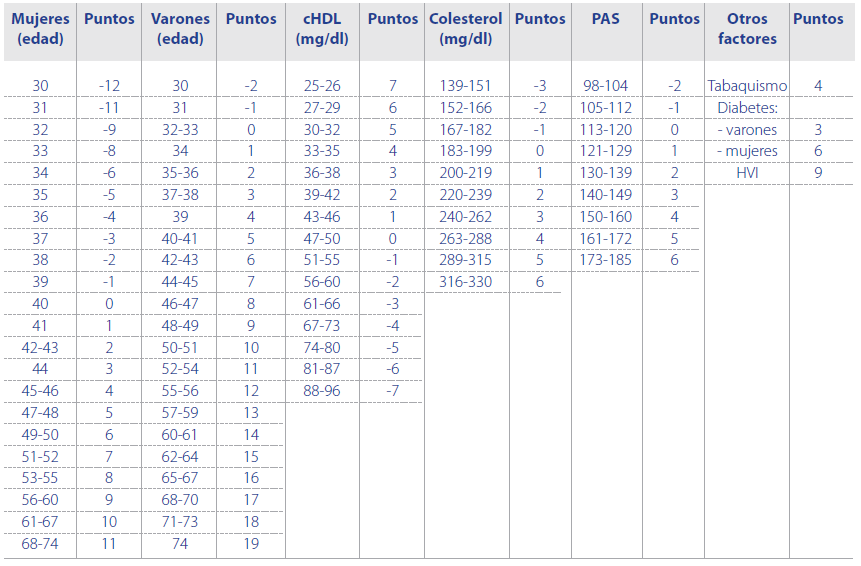
\includegraphics[width=\textwidth]{tablaFir} 
	\caption[Tabla Framighan]{Tabla de Predicción del RCV de Framingham (Anderson, 1991) \cite{tagle2007estimacion}
	}
	\label{fig:tablaFir1}
\end{figure}

\begin{figure}[htb]
	\centering
	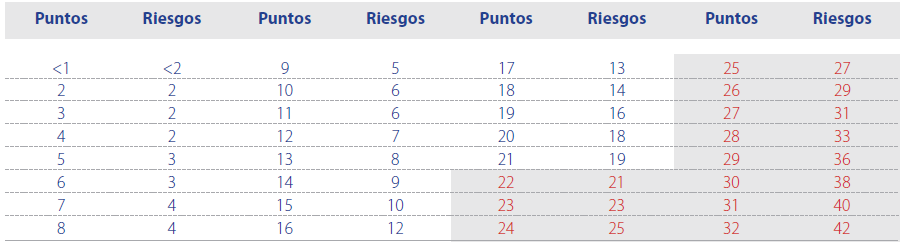
\includegraphics[width=\textwidth]{tablaFir2} 
	\caption[Predicción Framighan]{Predicción del RCV de Framingham (Anderson, 1991) \cite{tagle2007estimacion}
	}
	\label{fig:tablaFir2}
\end{figure}
	\chapter {Fase II: Diseño}
\label{cap:Fase II.Diseño}
En el diseño de sistemas informáticos se suelen usar las arquitecturas multinivel o programación por capas, en la que a cada nivel se le confía una misión simple. Para el desarrollo de nuestra aplicación nos hemos marcado como objetivo el desacomplamiento de las diferentes partes que componen el sistema: capa de presentación, capa de datos y capa de lógica de negocios. En este sentido, comenzamos el proyecto diseñando la interfaz de usuario, continuamos modelando la parte lógica y terminamos añadiendo persistencia de datos.

\section{Presentación. Prototipo de la GUI}

Una vez identificados los requisitos de la aplicación, nos hemos centrado en la creación de bocetos de baja fidelidad de la aplicación. En esta parte, nos hemos preocupado por el diseño de ventanas y posicionamiento de los controles, así como en el diseño de formularios y listados de información. Para ello, nos hemos basado en los conceptos teóricos vistos en la asignatura\textbf{\emph{ Interacción Persona-Ordenador}}, como empleo de metáforas, selección adecuada de colores y, sobre todo los aspectos relacionados con principios de usabilidad (flexibilidad, adaptabilidad, consistencia, etc.) y Leyes de Gestalt.

En este sentido, hemos utilizado la aplicación Balsamiq Mockups para realizar un prototipado horizontal que incluye la interfaz de todas las características del sistema, pero sin funcionalidad subyacente. En las capturas que se adjuntan a continuación, se incluyen los bocetos de baja fidelidad que creamos en una primera fase del proyecto, y que consecuentemente, pueden haber sufrido modificaciones con respecto al aspecto final de la aplicación. 


\subsubsection{Ventana de Inicio}
\begin{wrapfigure}{l}{0.3\linewidth}
    \centering
    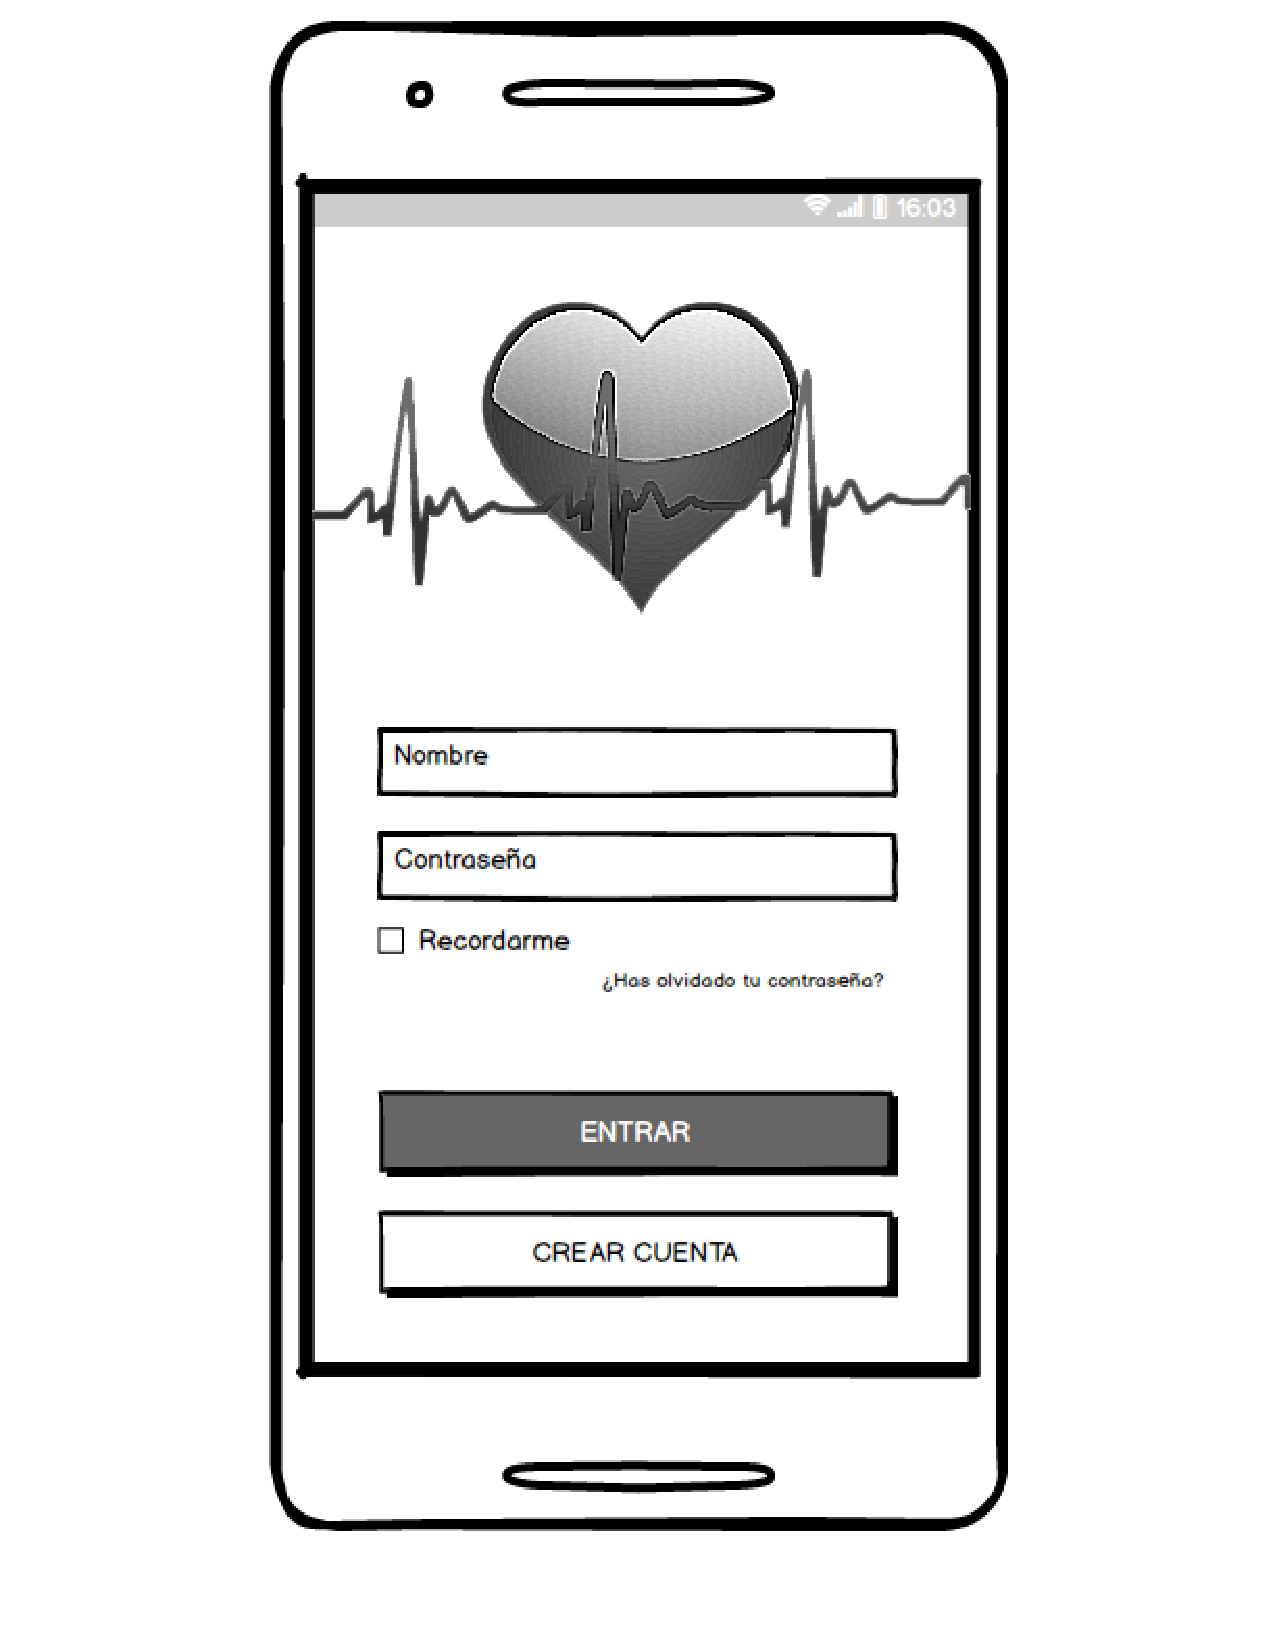
\includegraphics[width=1\linewidth]{GSI-1}
    \caption{{Ventana de Inicio}}
    \label{fig:GES1}
\end{wrapfigure}
Para que la aplicación permita monitorizar la evolución del RCV y pueda utilizarse como una herramienta motivacional para el paciente, hemos considerado obligatoria la necesidad de diseñar una ventana de \emph{login}, como paso previo a la utilización de las funciones de la aplicación. 

De esta forma, se podrá registrar cada uno de los cálculos realizados por el usuario y mostrar un gráfico con la evolución del RCV. Además, al disponer de cierta información personal sobre el usuario, no será necesario que introduzca algunos datos necesarios para realizar el cálculo.

Una vez autenticado, la navegación por la aplicación se basará en una barra de navegación situada en la parte inferior de la pantalla y que ofrecerá la posibilidad de desplazarse por tres ventanas: estado, nuevo cálculo y perfil. Una de las razones que nos llevan a tomar esta decisión de diseño, es que la barra de navegación inferior se encuentra dentro de la ‘thumb zone’, que es el área que puede alcanzar el usuario cuando sujeta el móvil con una sola mano utilizando el pulgar para navegar. De esta forma, permite navegar rápidamente entre las principales vistas del menú de la app. 

\subsubsection{Ventana de Estado}

\begin{wrapfigure}{r}{0.3\linewidth}
	\centering
	\subfigure[Ventana de Estado]{
			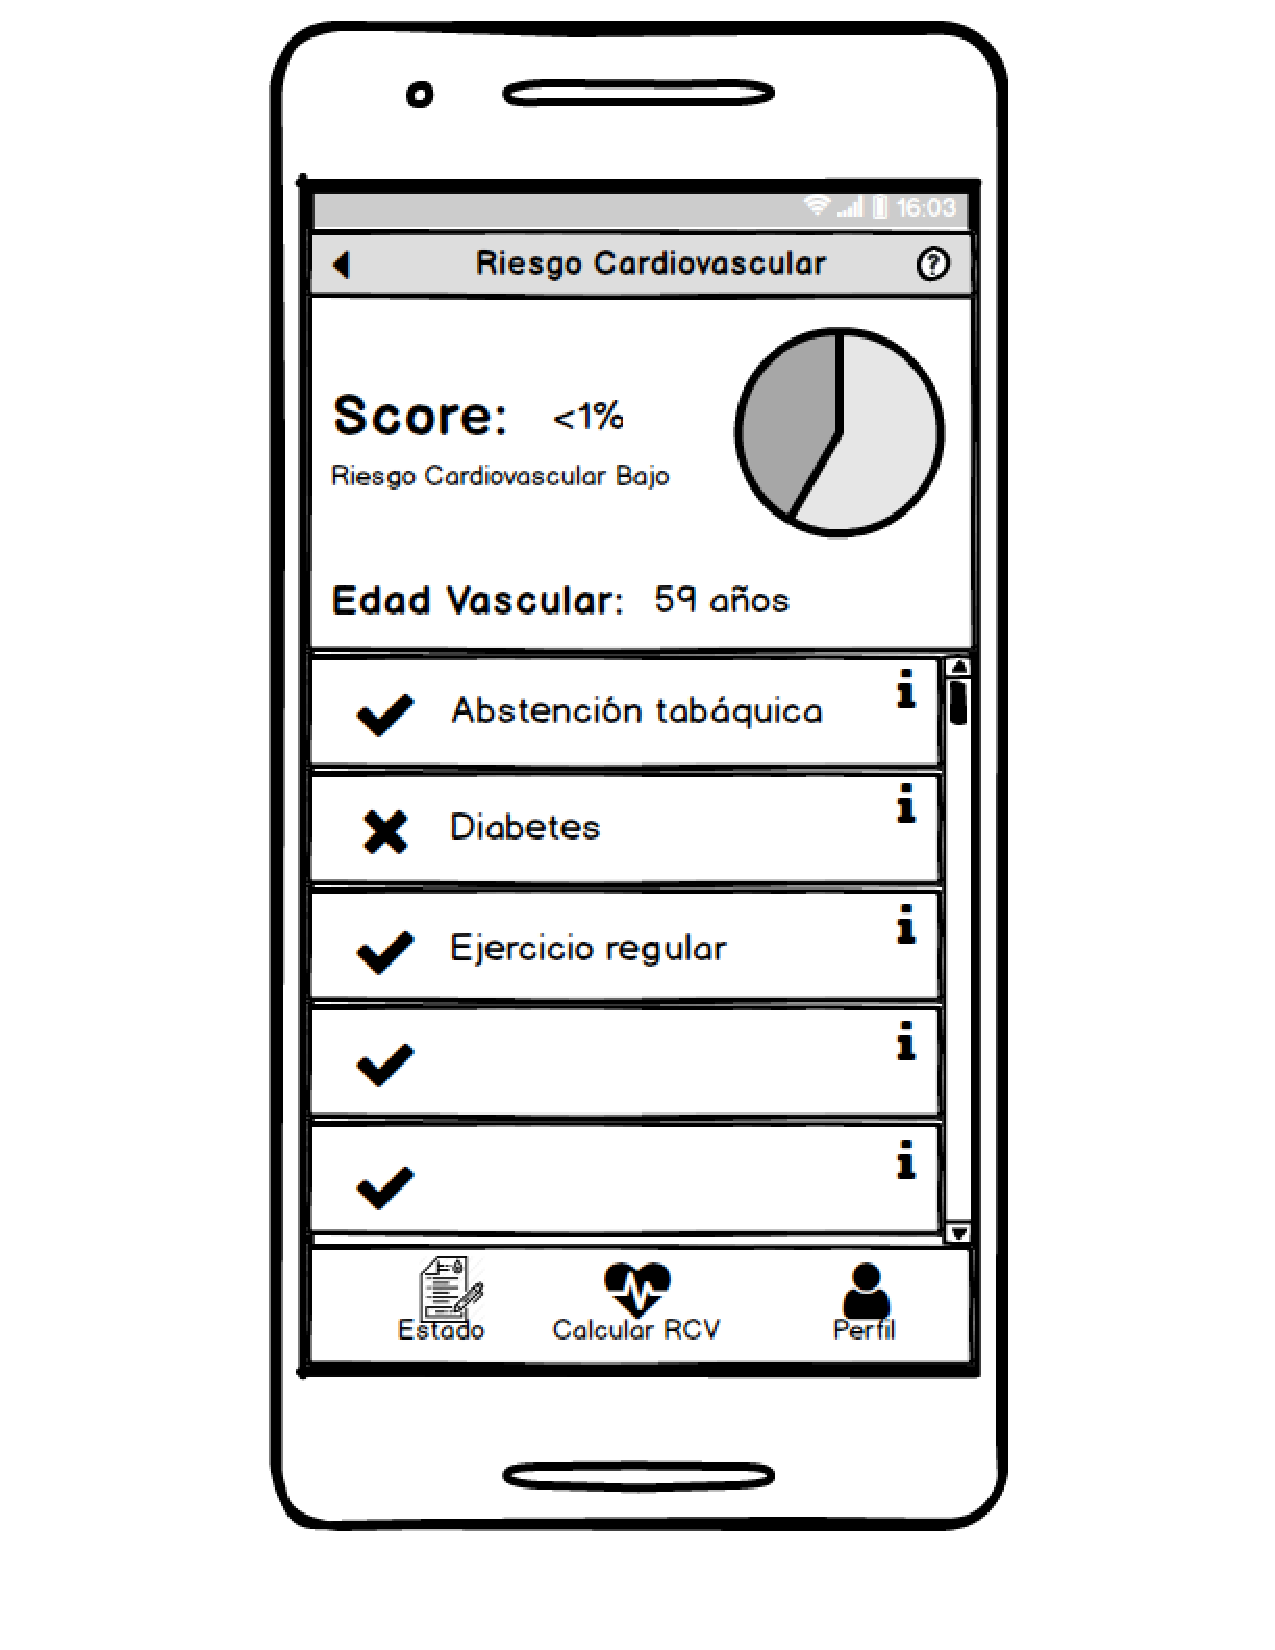
\includegraphics[width=0.3\textwidth]{GSI-2}
			\label{fig:graficoSE}
		}
		\subfigure[Ventana de Perfil]{
			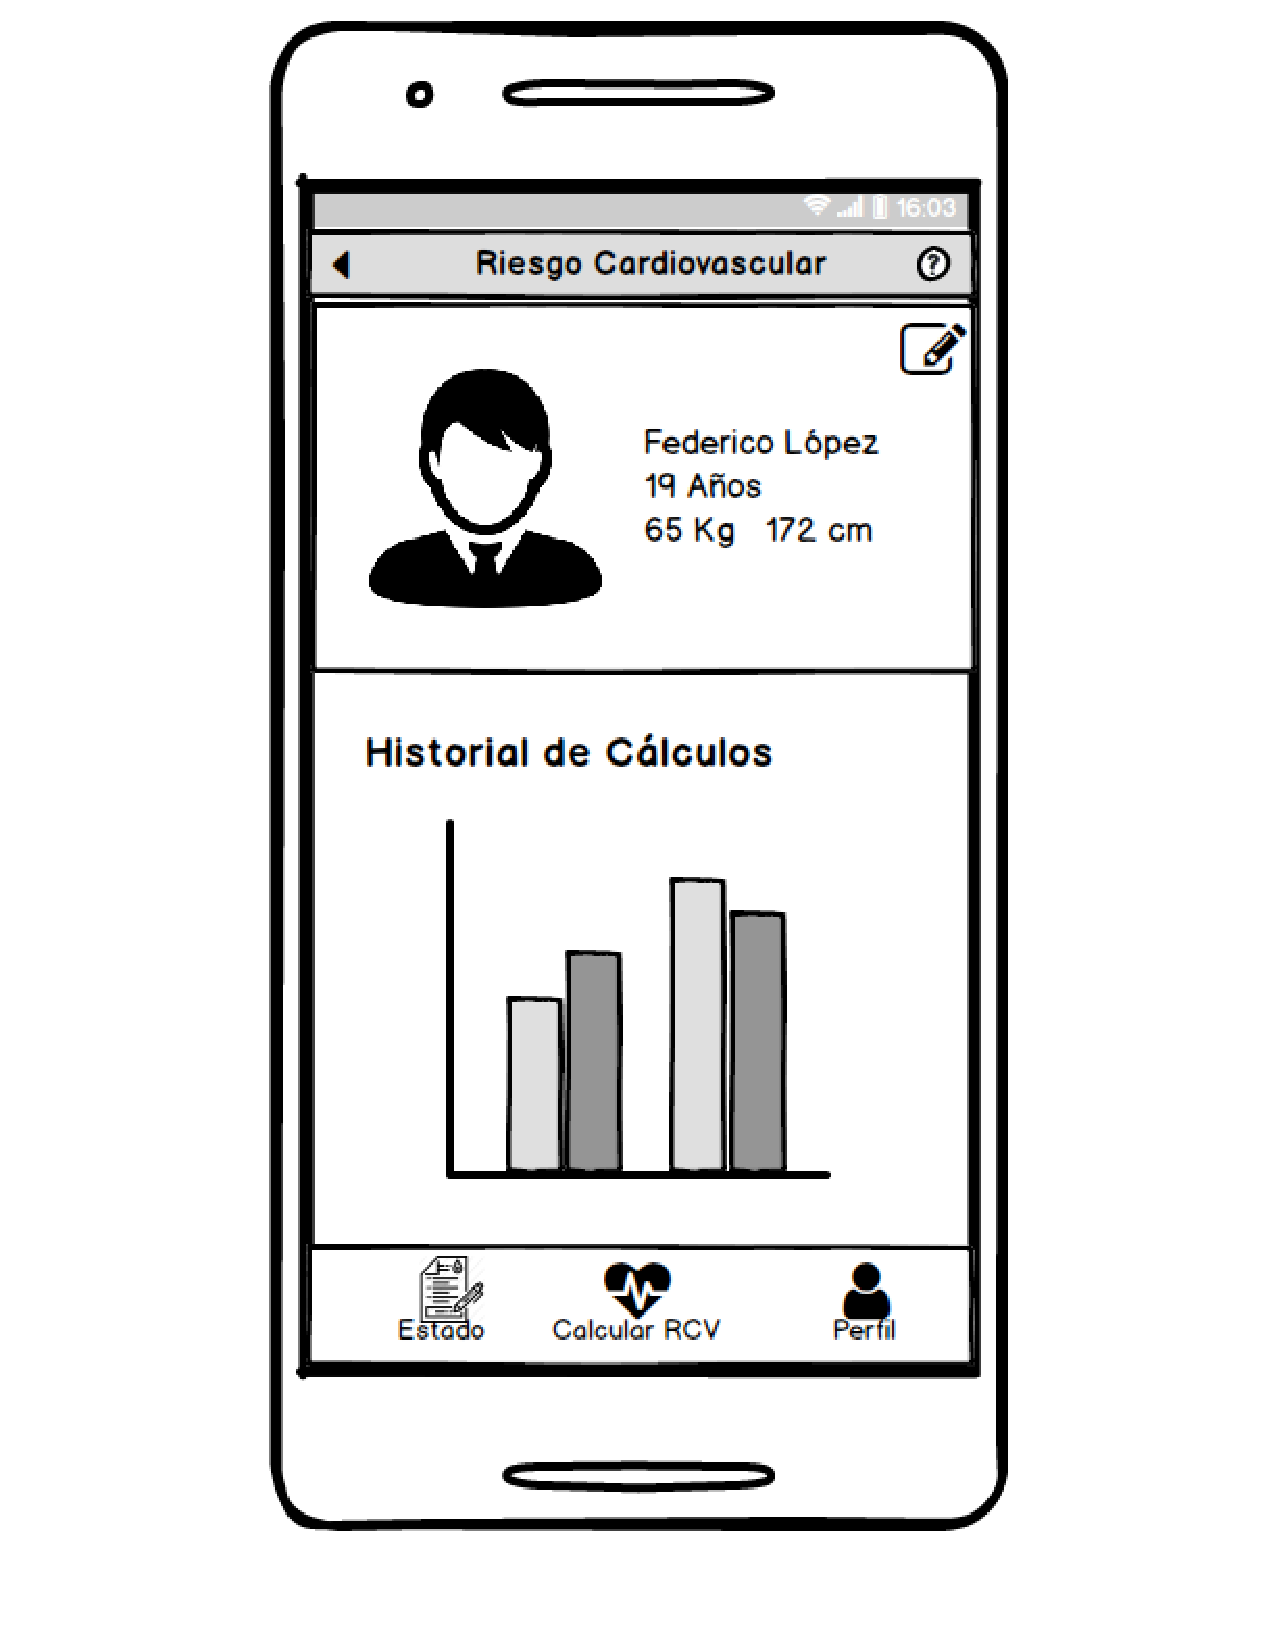
\includegraphics[width=0.3\textwidth]{GSI-3}
			\label{fig:tablaSE}
		}
		\caption[Ventana de Perfil y Estado]{Ventana de Perfil}
	
	\label{fig:defPerfil}
\end{wrapfigure}
La primera de las opciones seleccionables en el menú de navegación será la denominada Estado. En ella, se mostrará información relativa al último cálculo de RCV realizado por el usuario que ha iniciado sesión. Para ello, en la parte superior de la pantalla se mostrará un gráfico circular con el porcentaje de riesgo calculado y la fecha del mismo. Horizontalmente alineado con esta información aparecerá una etiqueta en la que se clasifique ese último cálculo en riesgo alto, moderado o bajo, de acuerdo con la tabla ~\ref{fig:tablaFir2}.

Por otro lado, se incluirá un listado dinámico con información sobre los factores de riesgo utilizados para realizar el cálculo. En este sentido, aparecerá información sobre la abstención o no de tabaco por parte del usuario, actividad física, tensión arterial, colesterol y si el usuario está en su peso ideal de acuerdo basándose en un cálculo del índice de masa corporal (IMC).


\subsubsection{Ventana de Perfil}
Lo más destacable de la ventana que se mostrará al seleccionar la opción del menú Perfil, es que se incluirá un gráfico que permita monitorizar la evolución del RCV. En el eje de las ordenadas se representará el porcentaje de riesgo cardiovascular, mientras que en el eje X se dimensionará la fecha en la que se realizó el cálculo.

Además del gráfico, en esta ventana se mostrarán los datos personales del usuario: nombre, apellidos, fecha de nacimiento y fecha de último acceso a la aplicación. 

\subsubsection{Ventana de Cálculo del RCV}
Seleccionando la opción Cálculo del menú de navegación de la aplicación el usuario podrá realizar una estimación del riesgo cardiovascular. Como sabemos, para poder aplicar el algoritmo de Framimgham, es necesario haber obtenido previamente una serie de información concreta relevante al usuario. Estamos haciendo referencia a los factores de riesgos de los que hablamos en la sección de Análisis (\ref{cap:Fase I. Análisis}). 

Esta ventana mostrará un formulario en el que se solicitará al usuario que introduzca su peso, altura, tensión arterial, si es o no fumador, colesterol (HDL y total), nivel de actividad física (un día por semana, dos días por semana, nada o una vez al mes) y enfermedades que puedan afectar al cálculo del RCV como la diabetes, hipertensión arterial o hipertrofia del ventrículo izquierdo.

\begin{figure}[htb]
	\centering
	\subfigure[]{
		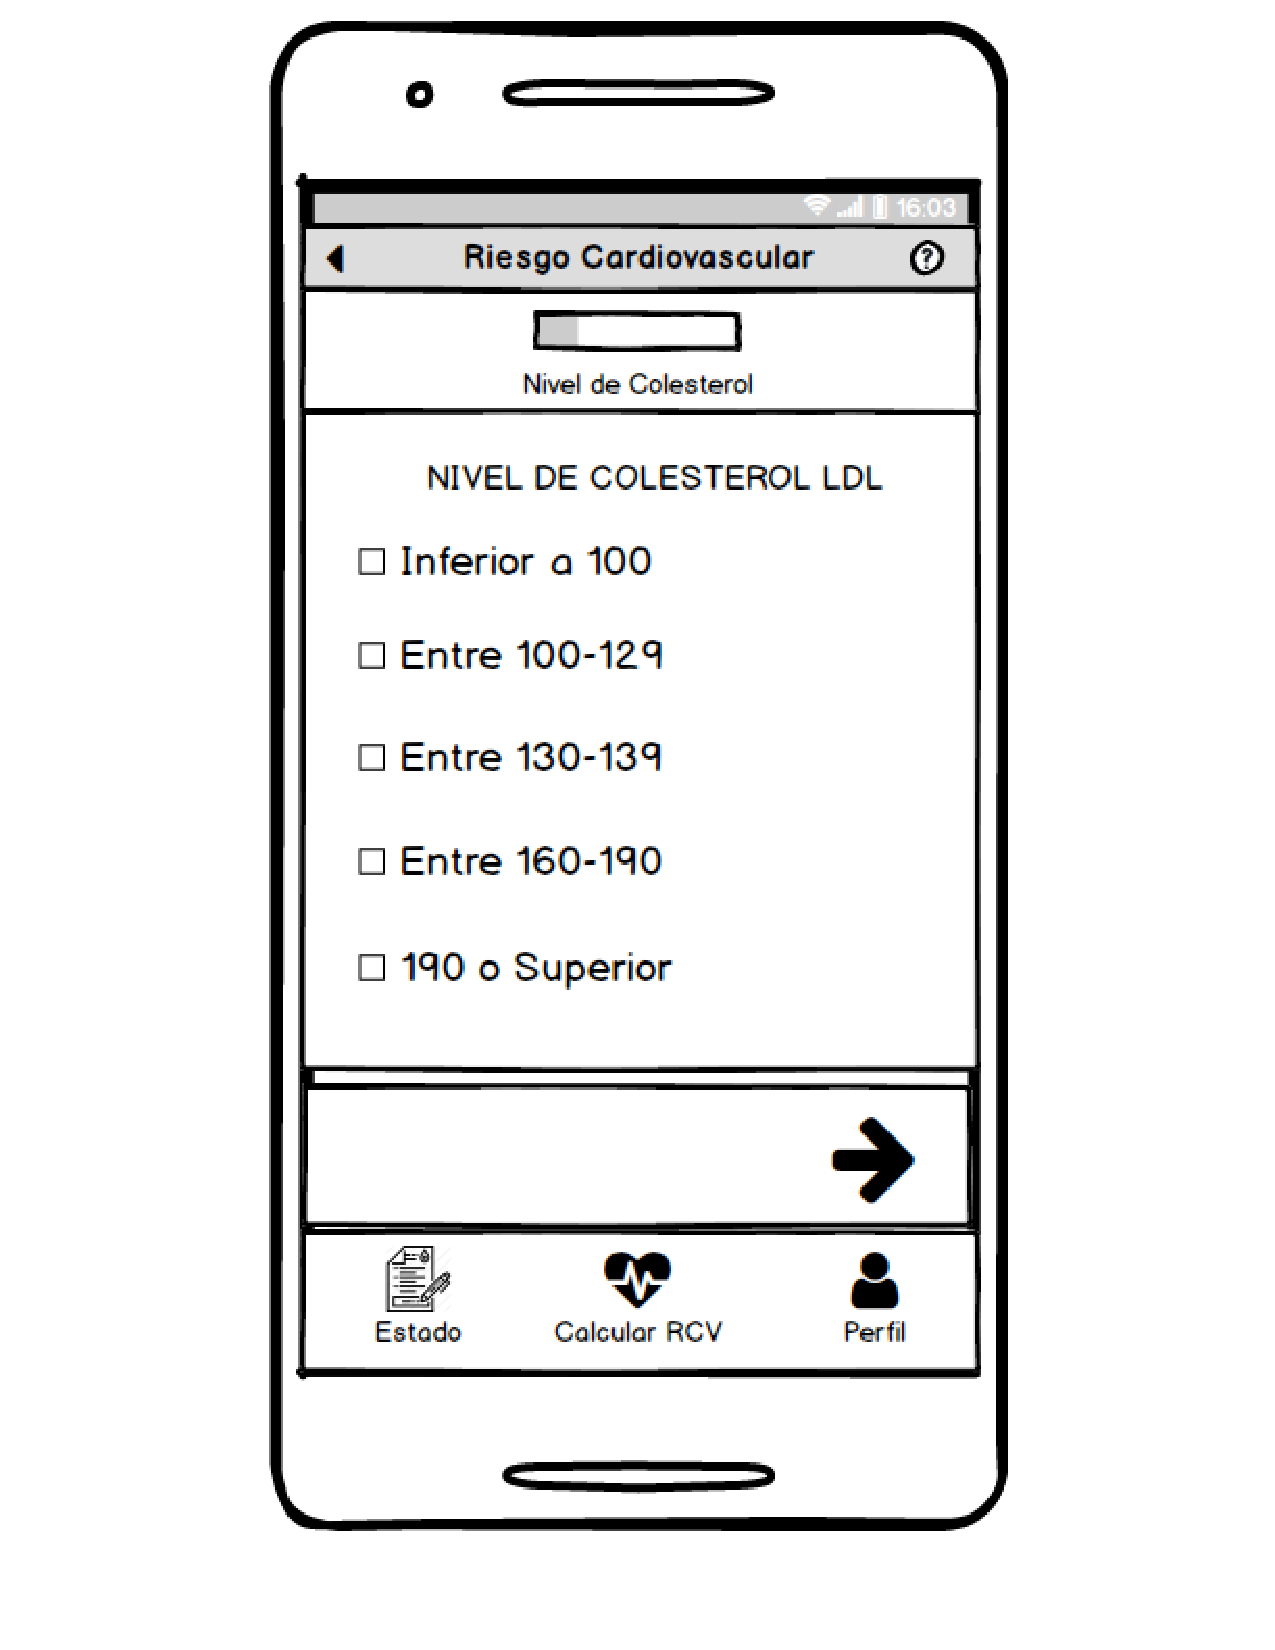
\includegraphics[width=0.3\textwidth]{GSI-4} 
		\label{fig:raCalculo1}
	}

		\subfigure[]{
			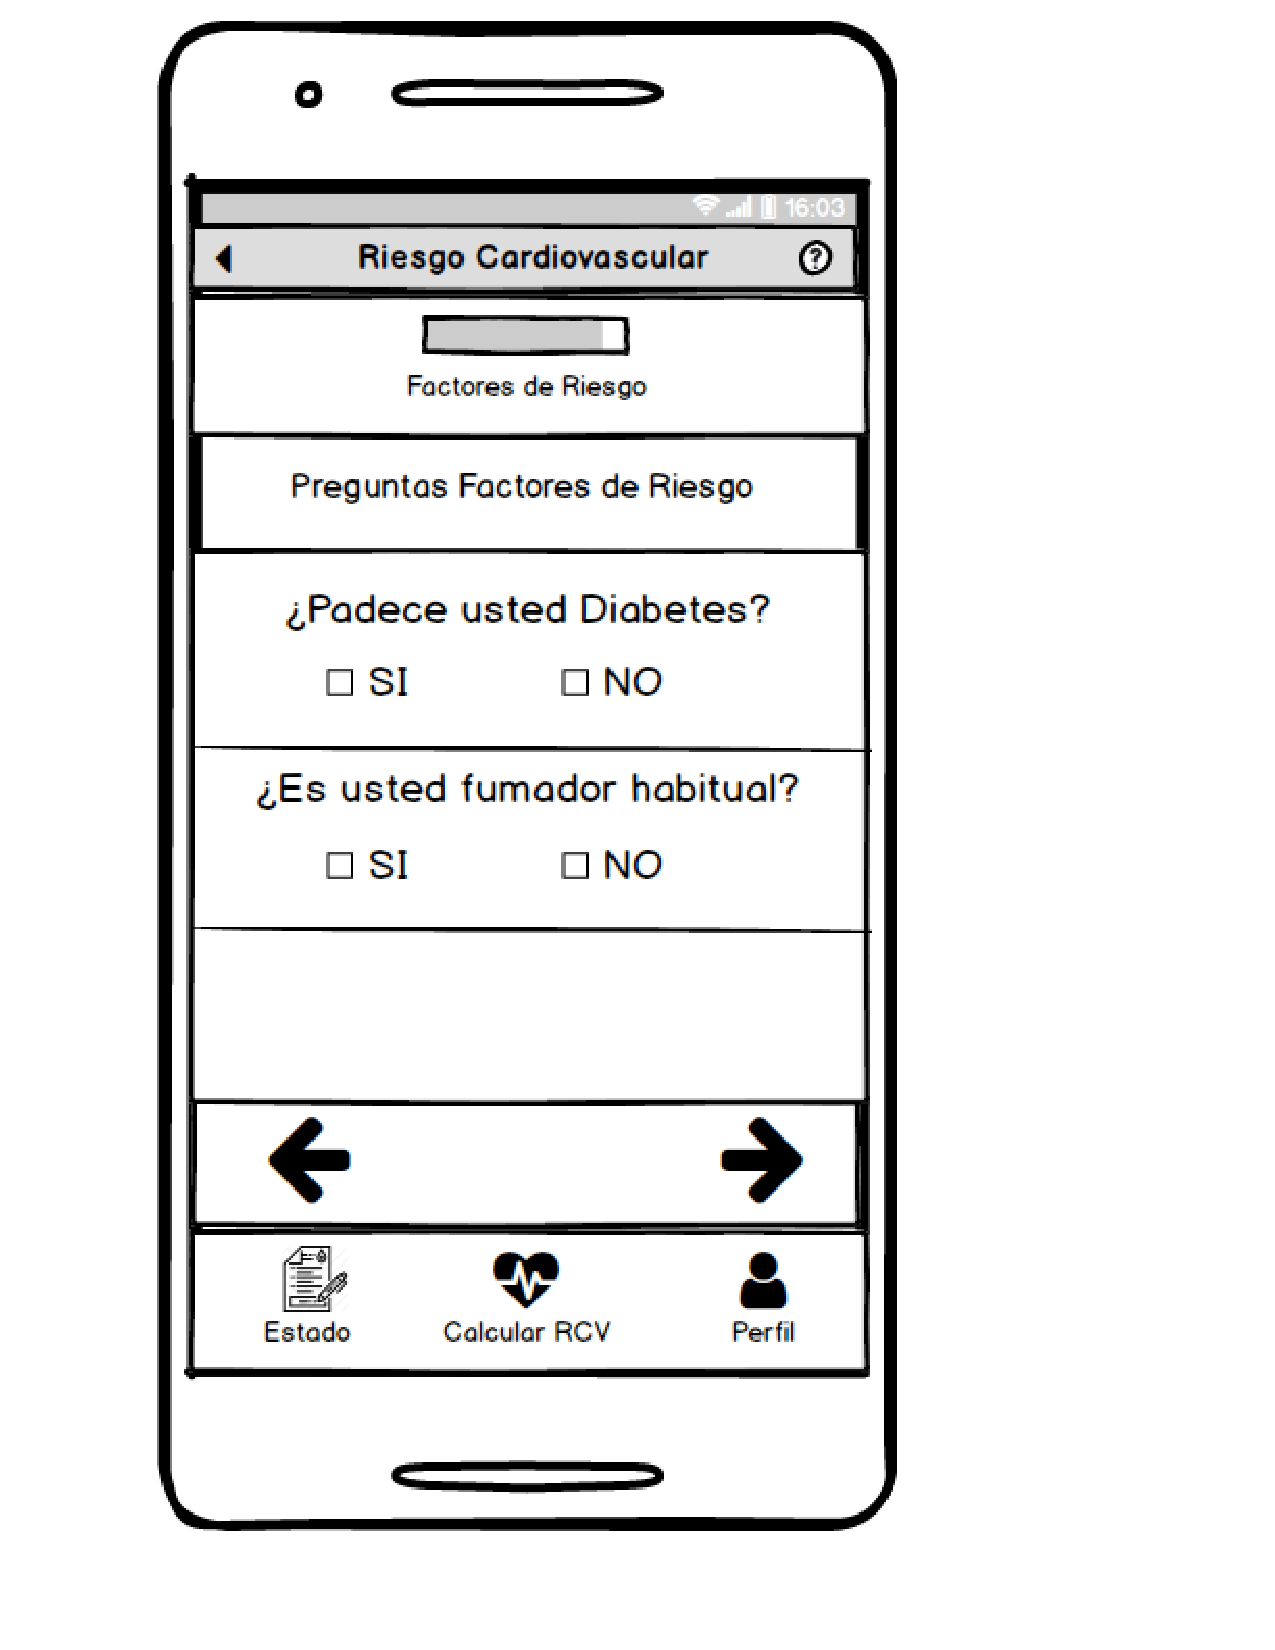
\includegraphics[width=0.3\textwidth]{GSI-9}
			\label{fig:raCalculo6}
		}
		\subfigure[]{
			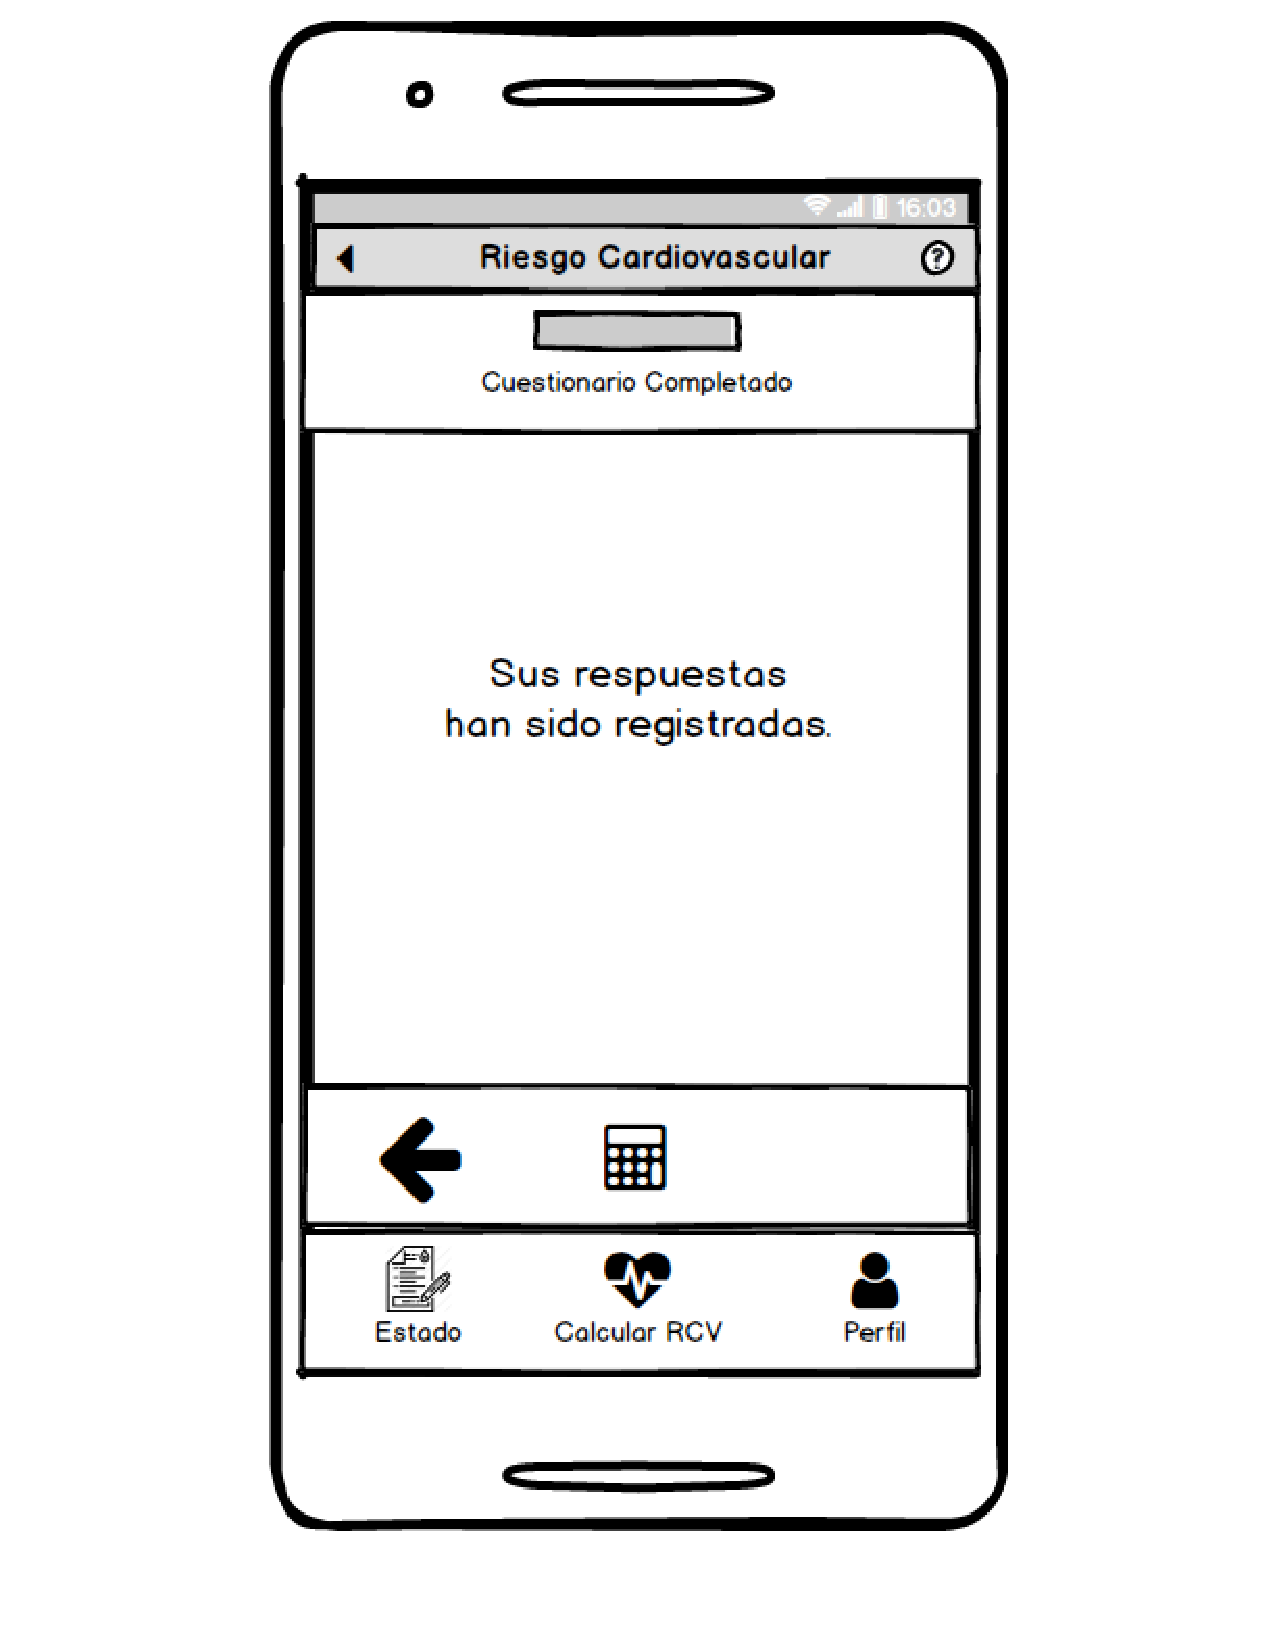
\includegraphics[width=0.3\textwidth]{GSI-10}
			\label{fig:raCalculo7}
		}
	\caption{Ventana Cálculo del RCV}
	\label{fig:cirugiaRA}
\end{figure}


\section{Dominio}
Dentro de la lógica de negocio, los usuarios se representan como objetos de la clase \emph{\textbf{Usuario}} con una serie de propiedades para realizar la autenticación: correo electrónico y pass. Además, para permitir el control de la evolución del RCV, cada objeto usuario almacena un \emph{array} con el historial de cálculos asociados a ese usuario. Un cálculo está definido mediante un objeto de la clase \textbf{\emph{CalculoRCV}}, la cual contiene atributos y métodos necesarios para encapsular una estimación de riesgo cardiovascular. Esta es la razón de la unión mediante una relación de asociación entre la clase Usuario y CalculoRCV.

Al mismo tiempo, la clase CalculoRCV contiene como atributo un objeto de la clase \textbf{\emph{FactoresRCV}}, la cual se utiliza para encapsular los factores de riesgo que se mostrarán en el listado dinámico que explicamos en la parte de presentación.


Por otro lado, hemos definido una \emph{interface} \textbf{\emph{ConstantesFactores}} para definir todas las propiedades constantes utilizadas para la estimación de RCV y recomendaciones de actuación. En este sentido, en esta interfaz definidos como constantes los valores límites para el colesterol, tensión y resultados del cálculo. Esta interfaz es implementada por las clases \emph{FactoresRCV} y \emph{CalculoRCV}.

Finalmente la clase \emph{\textbf{FraminghamRiskScore}} contiene los métodos necesarios para calcular el porcentaje de riesgo cardiovascular según las tablas de Framimgham. Adjuntamos el código Java en el anexo \ref{cap:AnexoA}.


\begin{figure}[H]
	\centering
	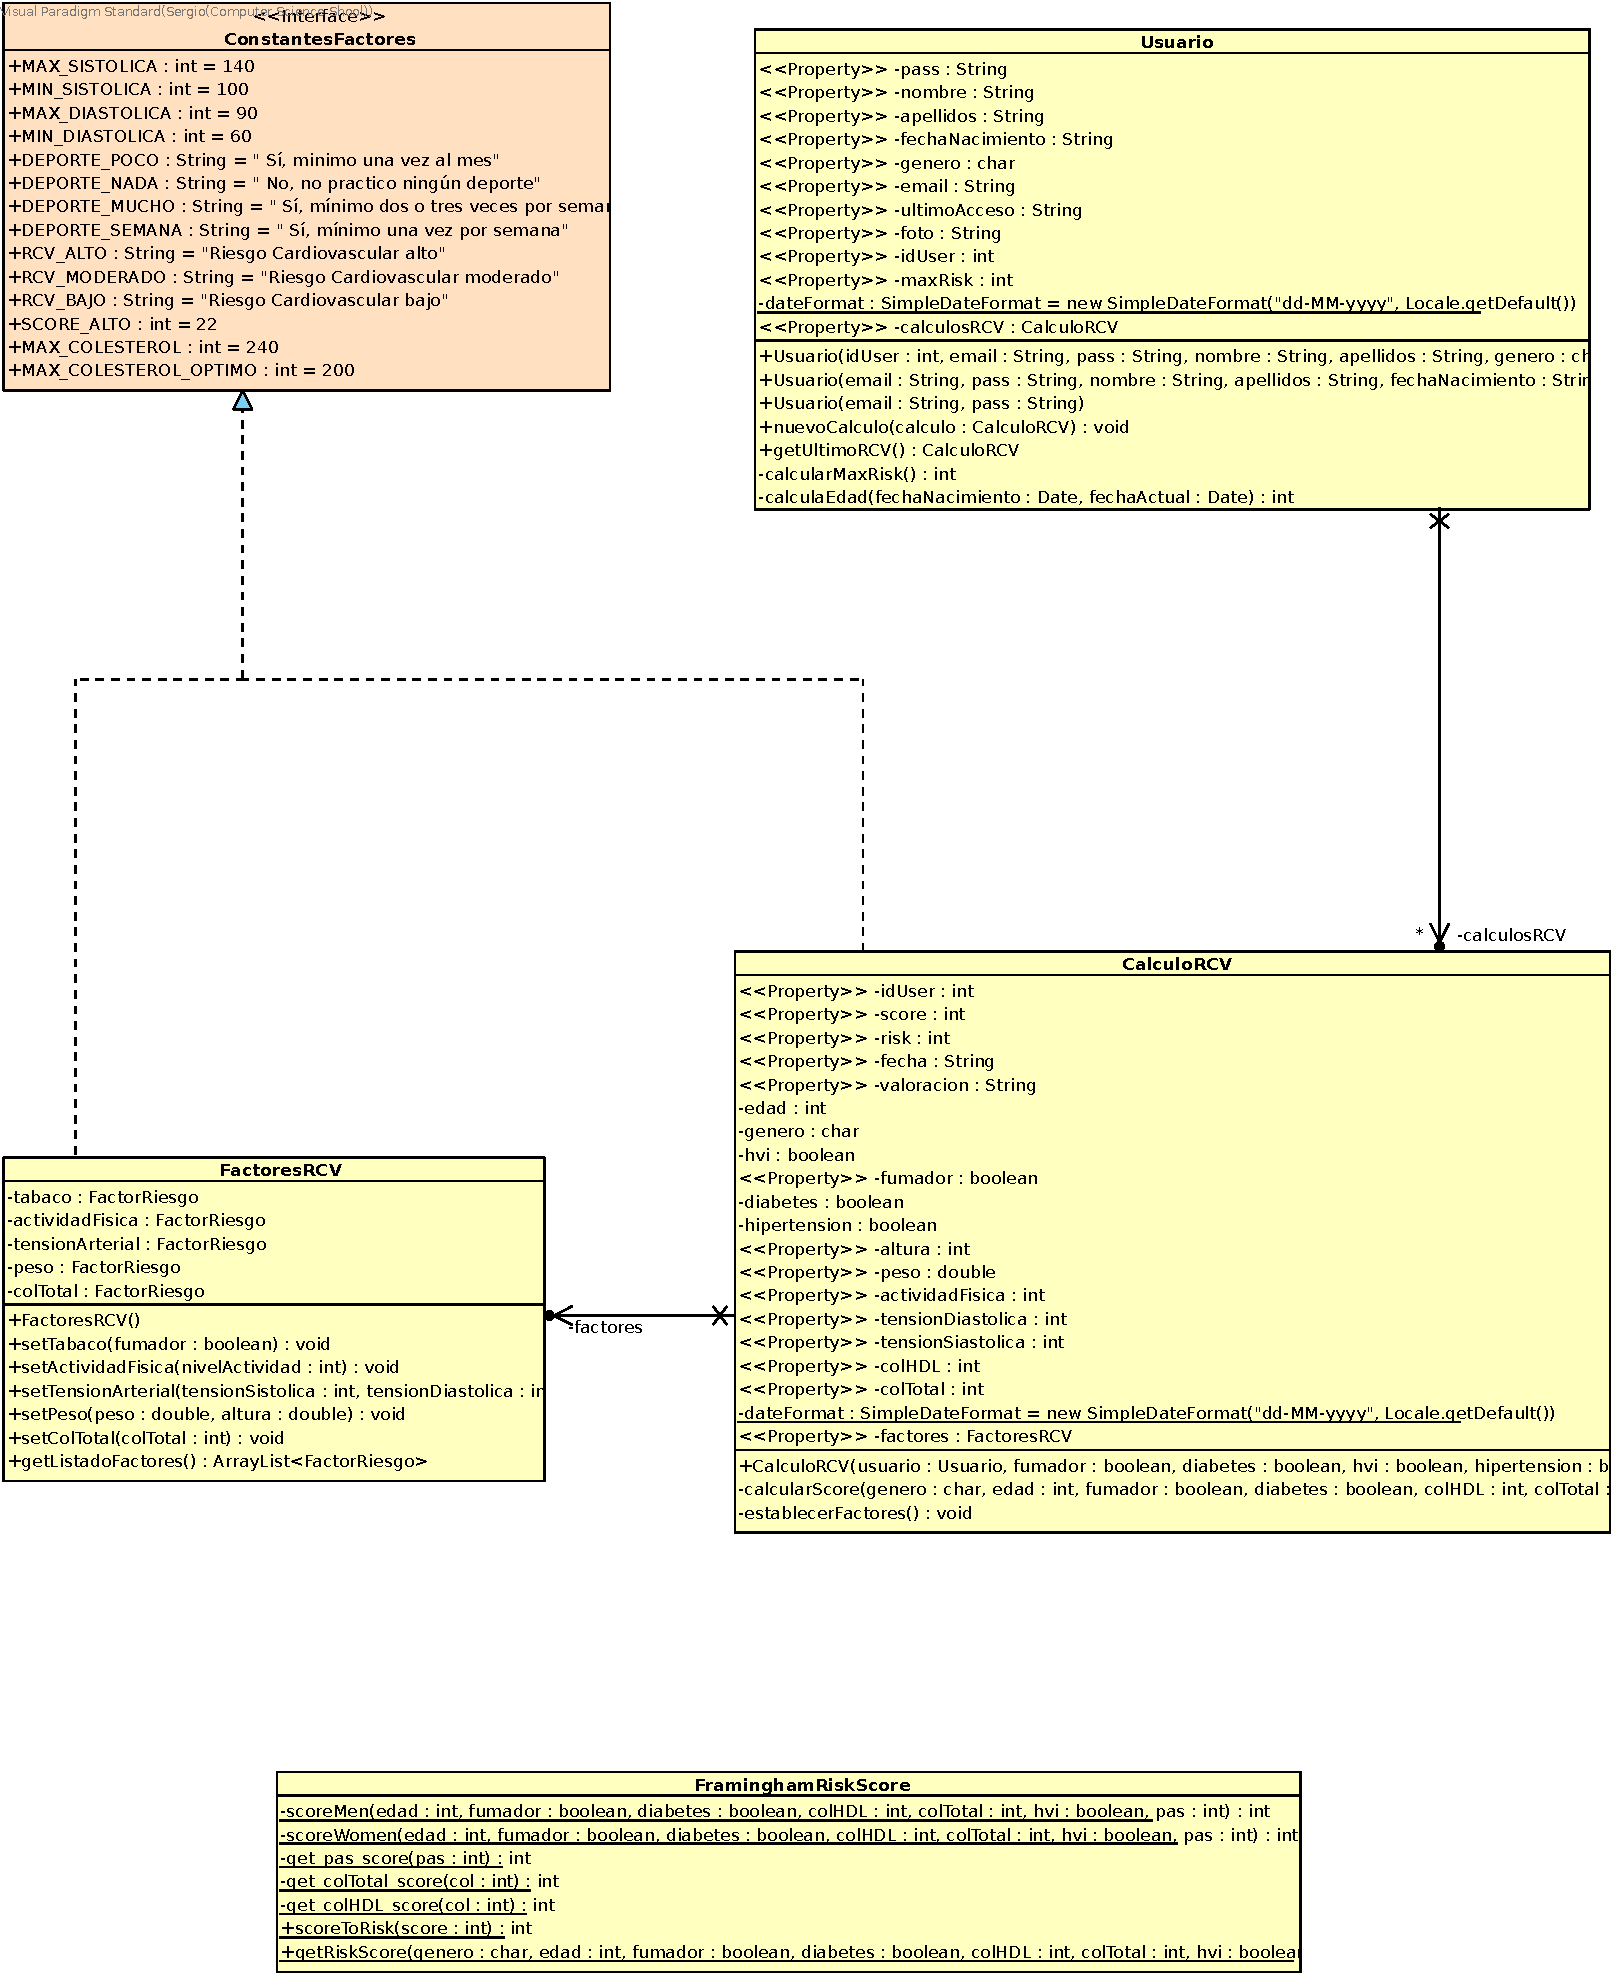
\includegraphics[width=\textwidth]{diagramClases} 
	\caption[Diagrama de clases]{Diagrama de clases UML de la capa de dominio
	}
	\label{fig:diagramaClases}
\end{figure}

\pagebreak



\section {Persistencia. BBDD Local}
Dentro de los distintos sistemas de bases de datos tanto privativos como libres/open source (Oracle, SQLServer, MySQL, etc) existe uno que se adapta perfectamente a las aplicaciones móviles:\textbf{ SQLite.} El principal motivo es que SQLite no requiere más que un simple fichero para almacenar los datos, ya que la lógica de funcionamiento debe ser implementada por la plataforma que desee interactuar con los datos.

\noindent Una vez decida la plataforma de BBDD que ibamos a utilizar en nuestra aplicación, era el momento de diseñar la estructura de la misma. Simplemente necesitamos modelar dos tablas: una para almacenar la información de los usuarios registrados en el sistema, indexada por un identificador único de usuario; y otra tabla en la que se almacenen todos los cálculos realizados en el sistema. Las dos tablas están relacionadas a través del identificador de usuario. 

Las siguientes imágenes muestran el código SQL de creación de las dos tablas que forman la base de datos de nuestra aplicación. 

\begin{figure}[htb]
	\centering
		\subfigure[Tabla Usuario]{
			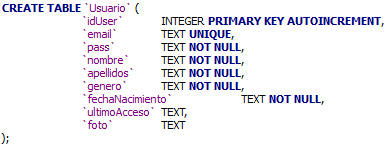
\includegraphics{userTabla}
			\label{fig:tablaUsuario}
		}
	\subfigure[Tabla CalculosRCV]{
		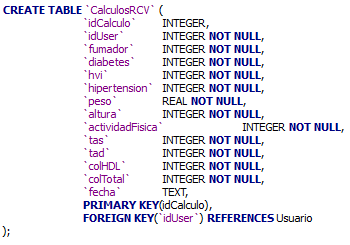
\includegraphics{calculoTabla}
		\label{fig:tablasCalculos}
	}

	\caption{Código creación de tablas SQLite}
	\label{fig:sqlite}
\end{figure}

\subsubsection{Implementación en Android}
El procedimiento recomendado para crear una nueva base de datos SQLite en Android, se resume de forma esquemática:
\begin{itemize}
\item Crear una \textbf{clase} que extienda de \textbf{\emph{SQLiteOpenHelper}}. En nuestro caso, la hemos llamado \emph{DB\_Helper}.

\item Sobreescribir en ella el método \textbf{\emph{onCreate()}}, donde se ejecutará un comando SQLite para crear las tablas de la base de datos.

\item También es necesario sobrescribir el método \textbf{\emph{onUpgrade}}, el cual se ejecutará cada vez que cambiamos la versión de la base de datos, y se usará para migrar los datos de la base de datos anterior a la nueva versión. 
\end{itemize}

El siguiente listado de código muestra los métodos \emph{onCreate} y \emph{onUpgrade} de la clase DB\_Helper, utilizada como conector en nuestra aplicación. 

\lstinputlisting[style=Java-color,caption={Clase DB\_Helper.java},label=lst:codCfile]{./code/DB_Helper2.java}





	\chapter{Fase III: Implementación}
\label{cap:Implementacion}

\section{Inicio de sesión y registro de un nuevo usuario}

\begin{figure}[H]
	\centering
	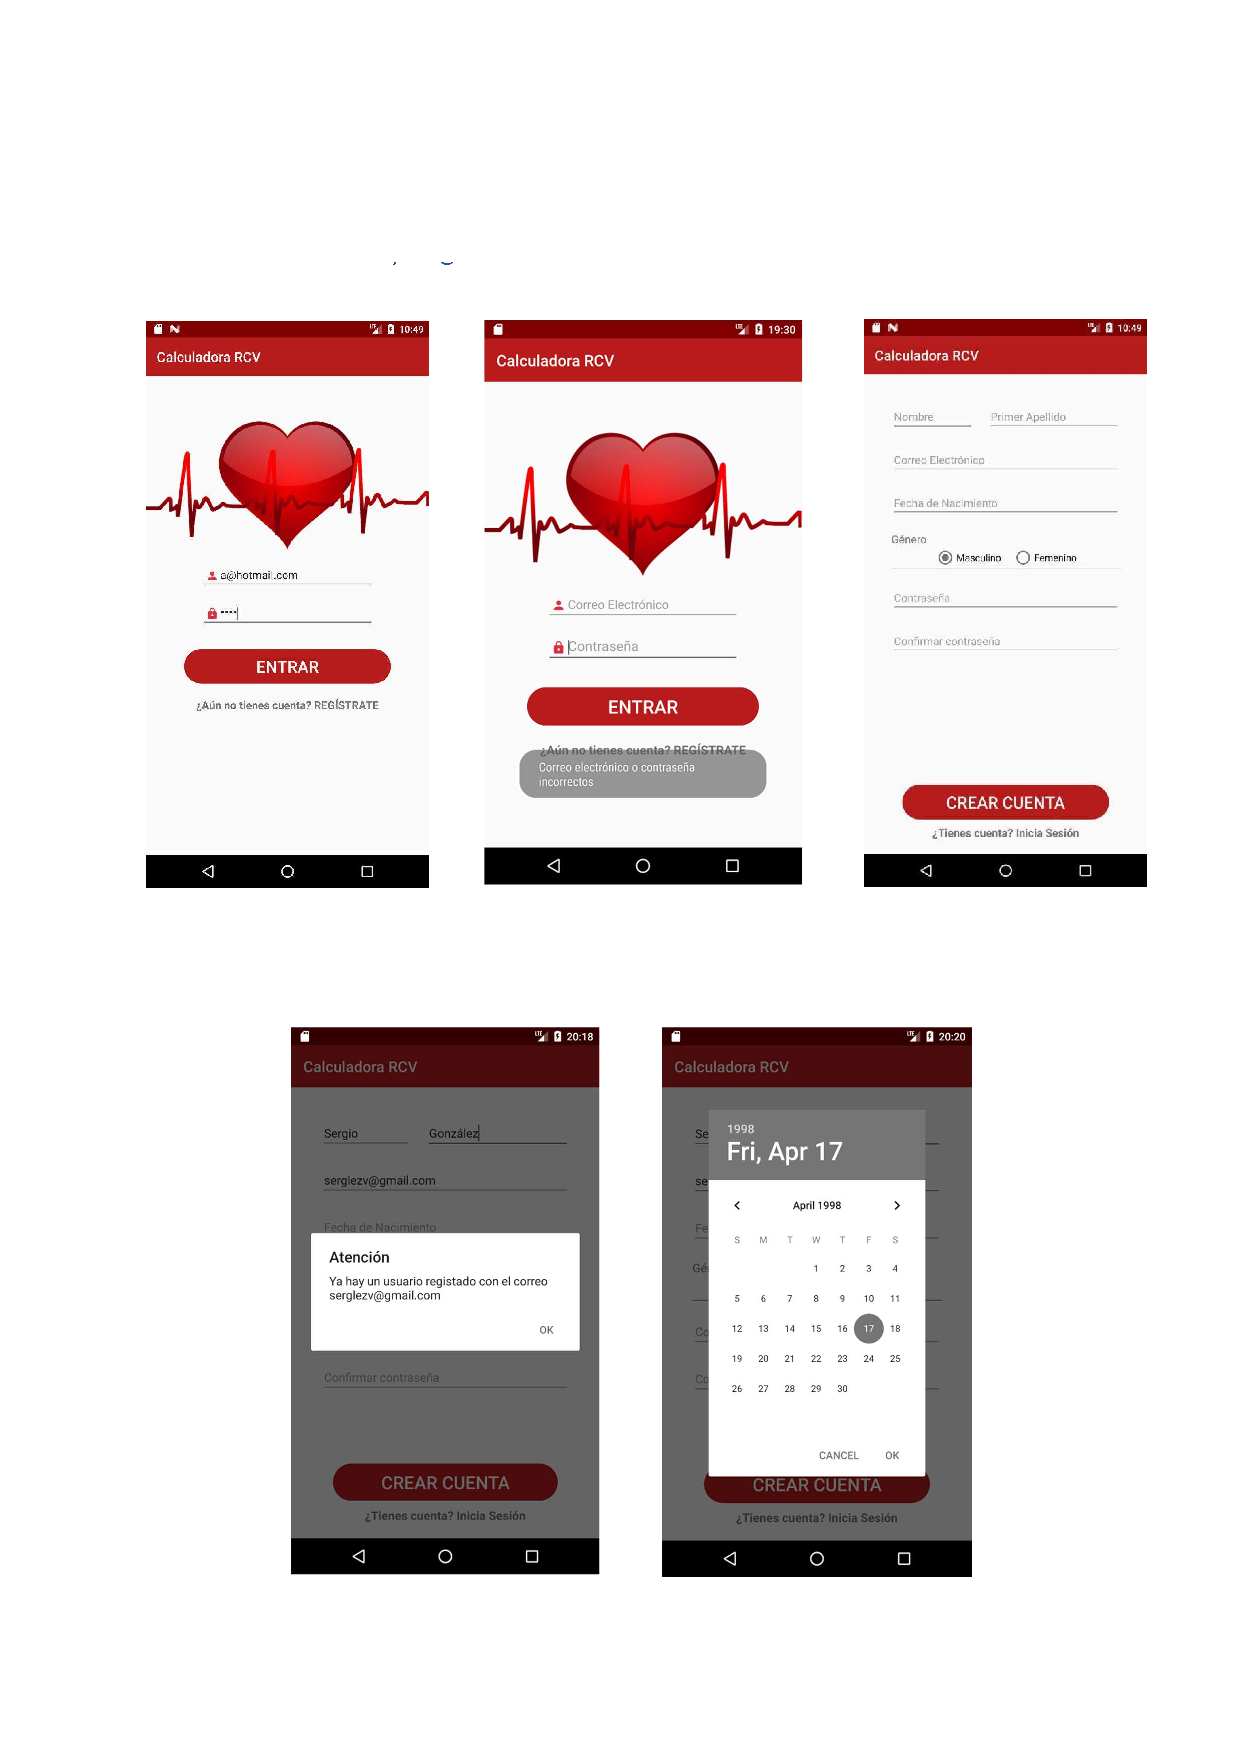
\includegraphics[width=0.9\textwidth]{loginRegistro} 
	\caption[loginRegistro]{Implementación de la ventana para iniciar sesión y registrarse.}
	
	\label{fig:loginRegistro}
\end{figure}



\section{Barra de navegación inferior}

\subsection{Ventana de Estado}
\begin{figure}[H]
	\centering
	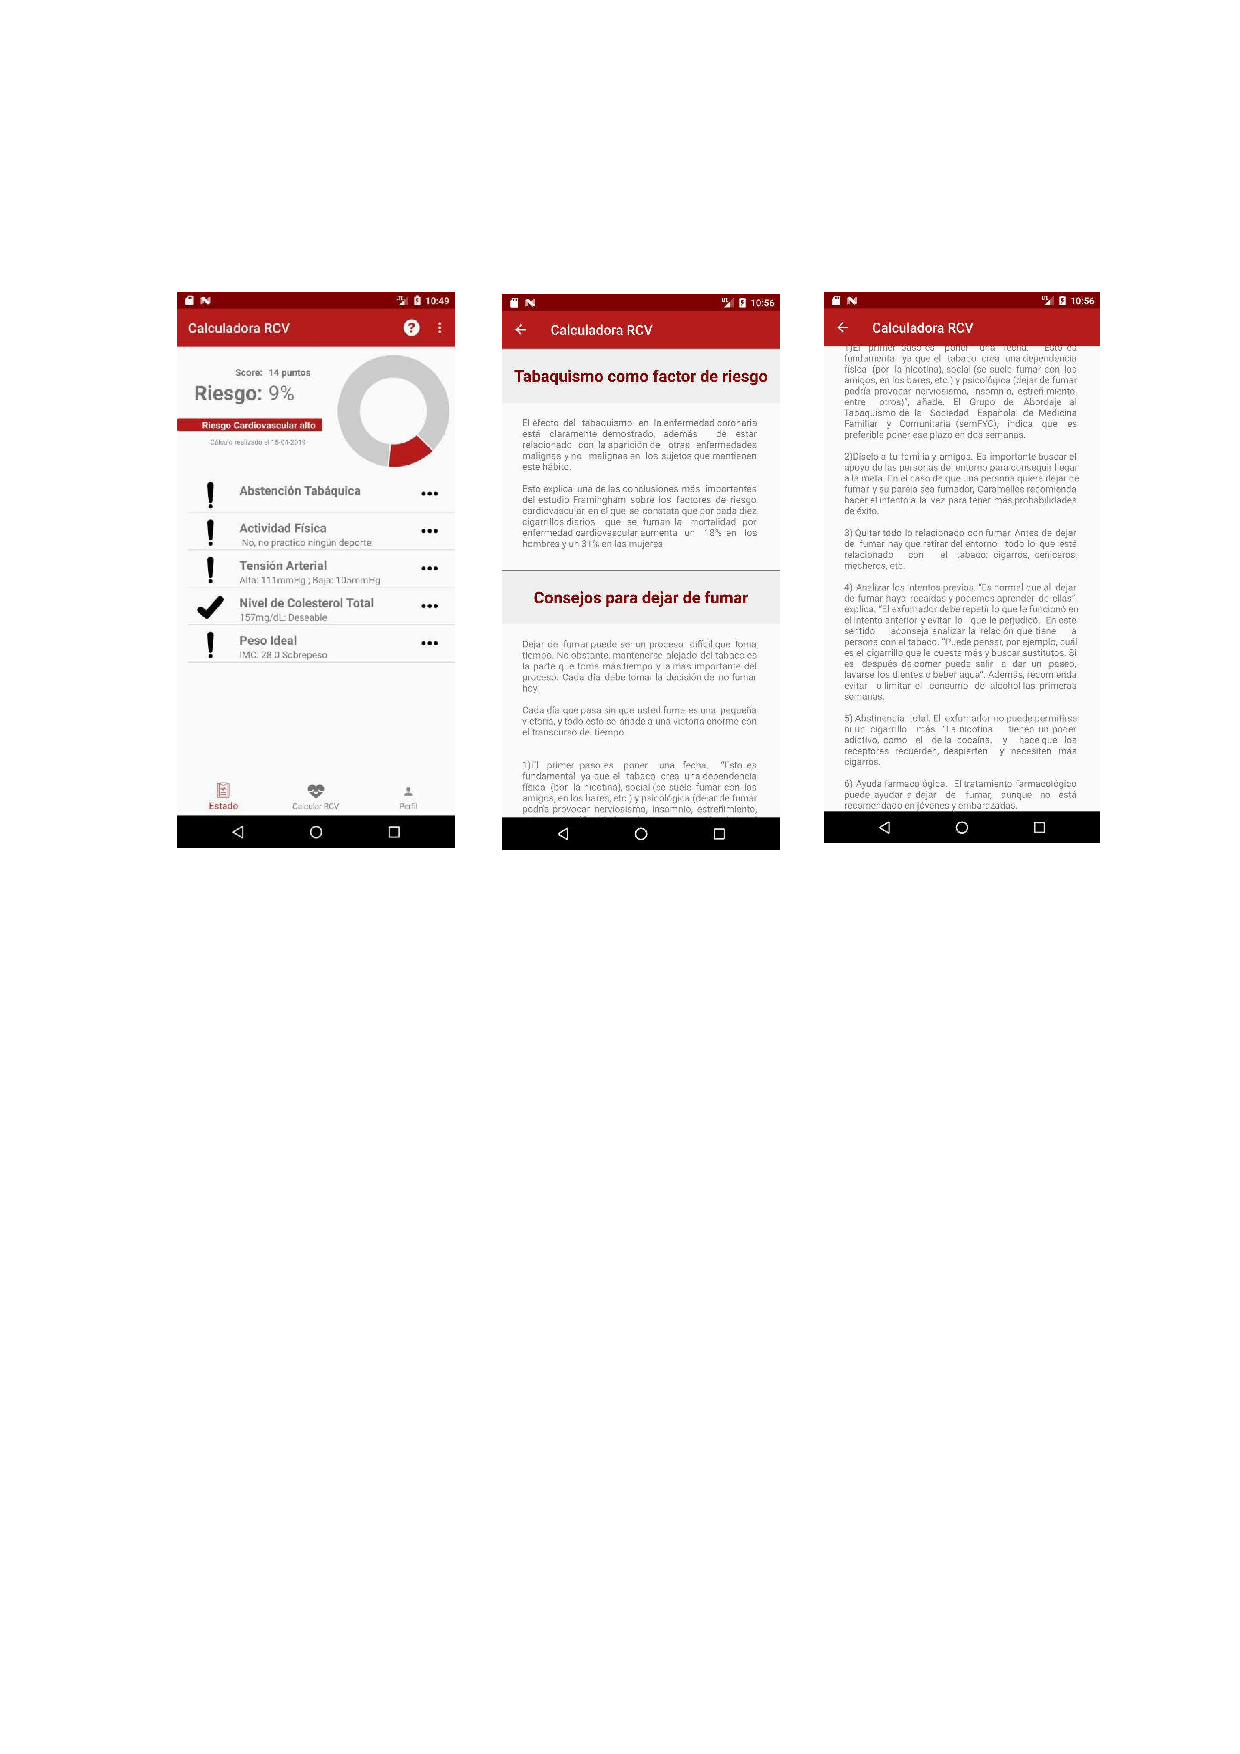
\includegraphics[width=0.9\textwidth]{ventanaEstado} 
	\caption[Implementación Estado]{Implementación de la ventana que informa sobre la última estimación de RCV realizada}
	
	\label{fig:ventanaEstado}
\end{figure}
\subsection{Ventana de nuevo Cálculo}
\begin{figure}[H]
	\centering
	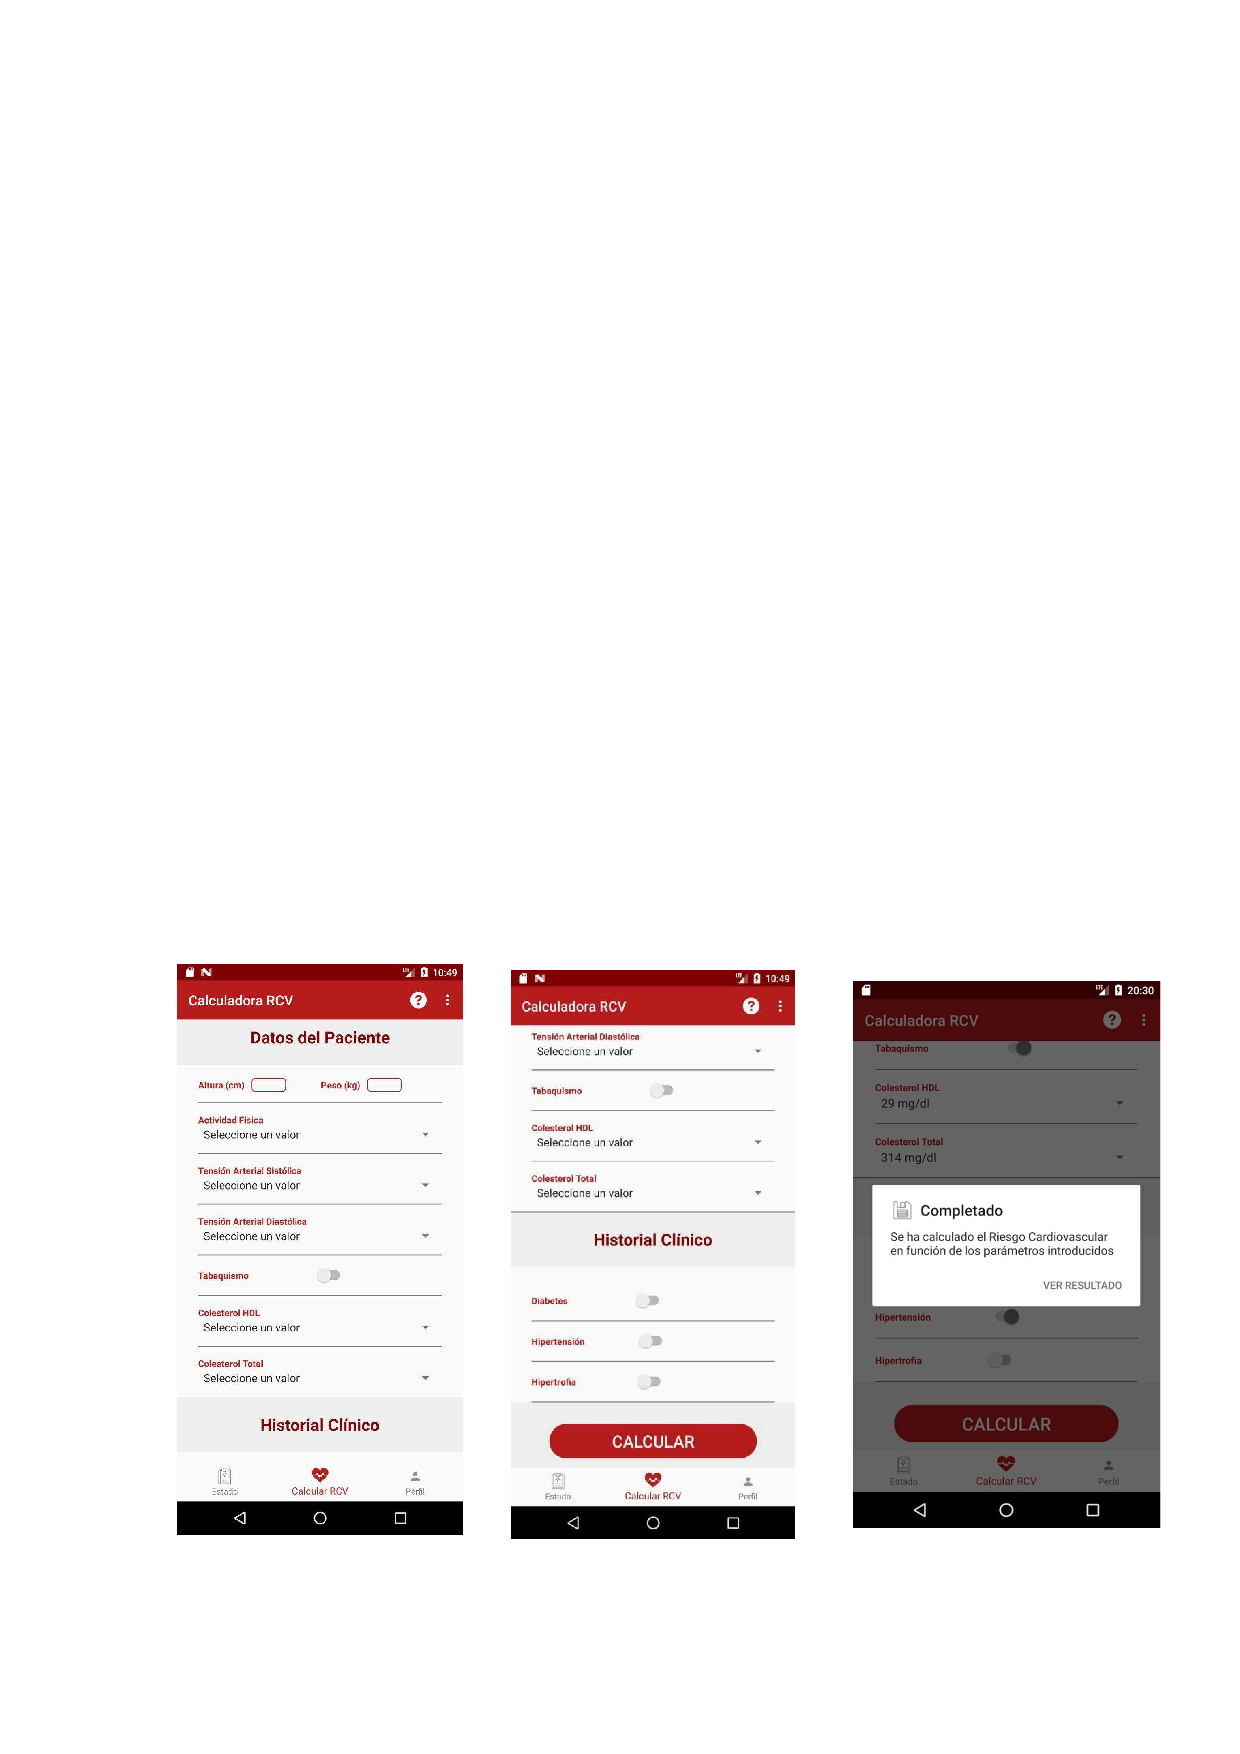
\includegraphics[width=0.9\textwidth]{ventanaCalculo} 
	\caption[Implementación Calculo]{Implementación del formulario para realizar un nuevo cálculo de estimación RCV}

	\label{fig:ventanaCalculo}
\end{figure}
\subsection{Ventana de Perfil}
\begin{figure}[H]
	\centering
	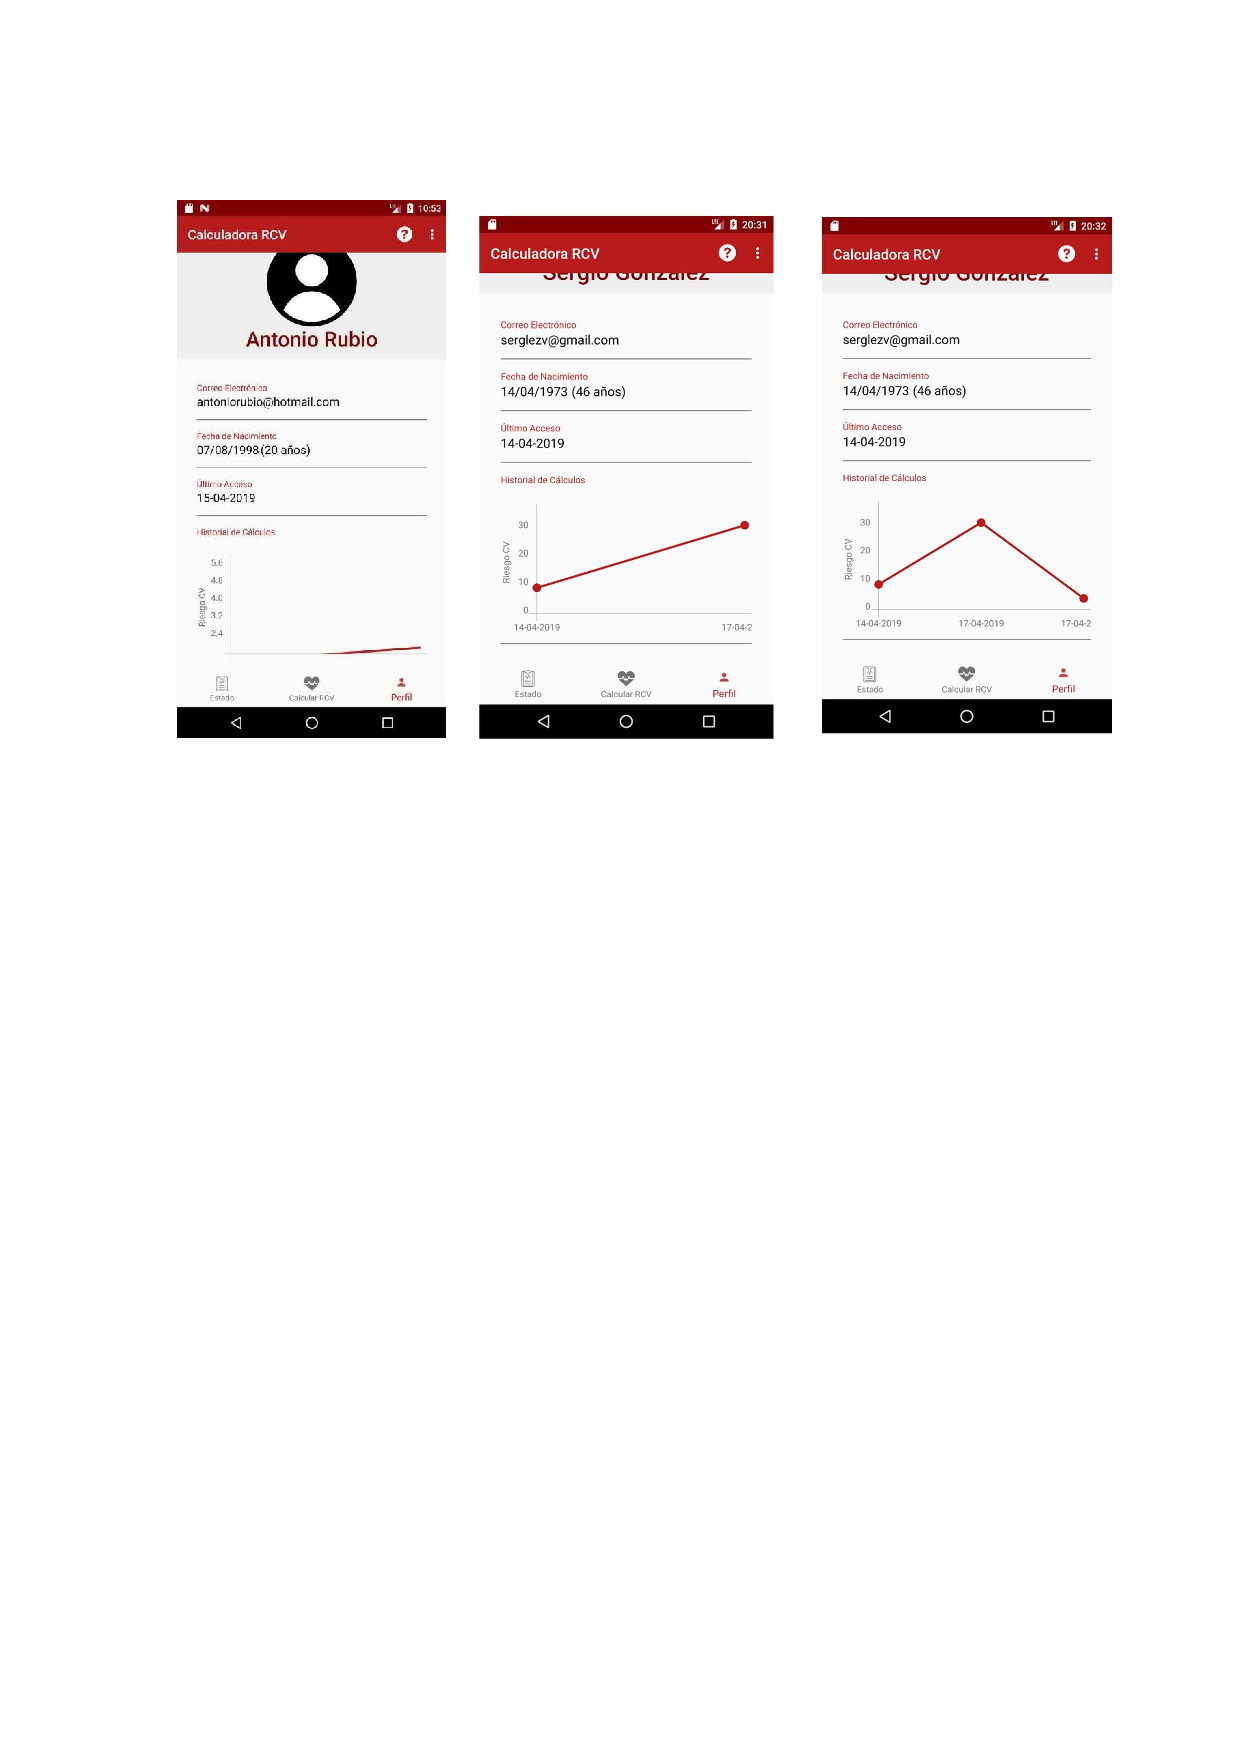
\includegraphics[width=0.9\textwidth]{ventanaPerfil} 
	\caption[Implementación Perfil]{Ventana de perfil en la que se muestra un gráfico que permite monitorizar la evolución del RCV}
	
	\label{fig:ventanaPerfil}
\end{figure}

\section{Action Bar y Acerca De…}
\begin{figure}[H]
	\centering
	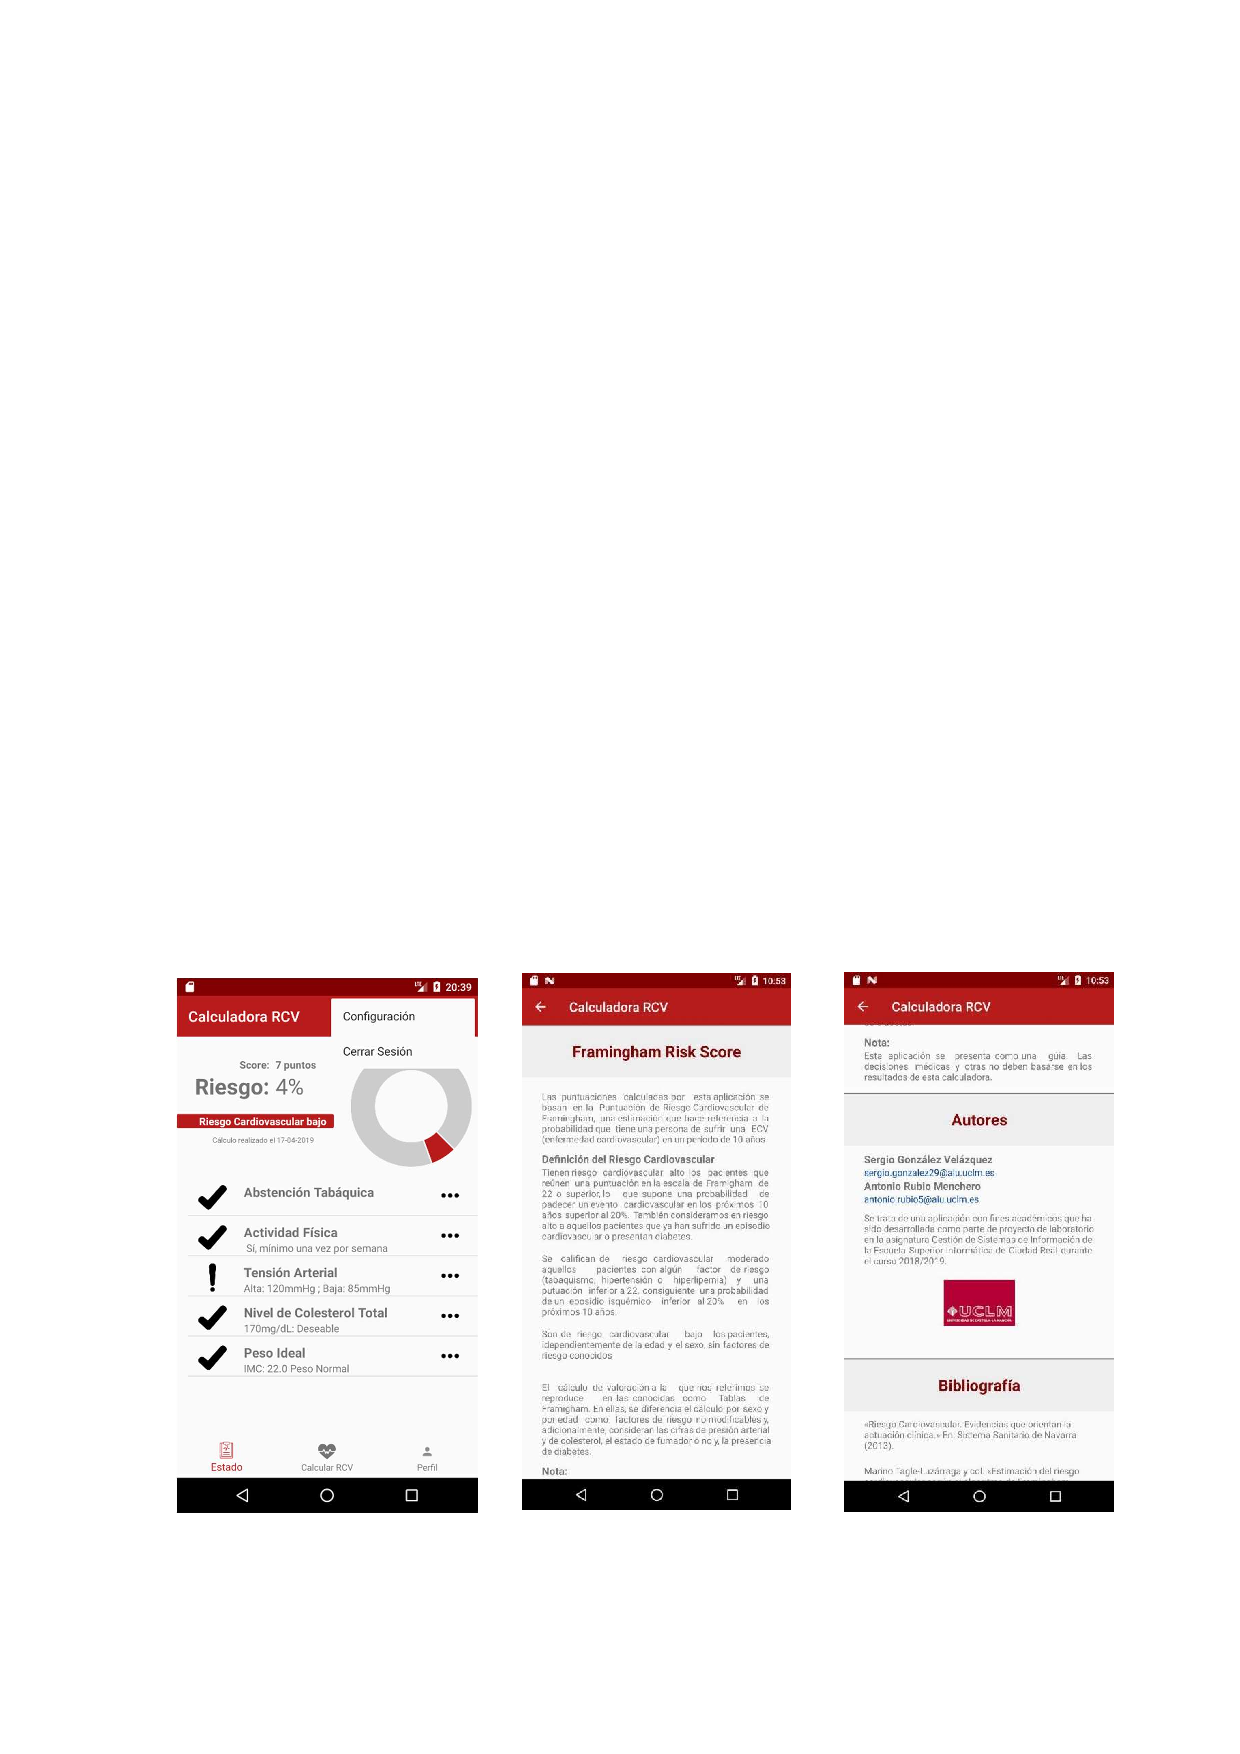
\includegraphics[width=0.9\textwidth]{ventanaActionBar} 
	\caption[Implementación Estado]{Ventana de información y ayuda sobre la aplicación}
	
	\label{fig:ventanaBar}
\end{figure}


	% -------------------------
	%
	% ANEXOS
	%
	% -------------------------
	\appendix
	
	% Tras este punto los capítulos se numeran con letras.
	% Aquí todos los apéndices necesarios
	\chapter{Tablas de Framingham en Java}
\label{cap:AnexoA}

Consideramos interesante incluir en la documentación de nuestra aplicación la implementación del algoritmo de Framimgham en Java. Para su desarrollo nos hemos basado en las tablas de estimación de riesgo cardiovascular explicadas en el capítulo \ref{cap:Fase I. Análisis}. Entrando un poco en detalle en la estructura de la clase \textbf{FramighamRiskScore}, cabe destacar la existencia de los métodos públicos \emph{\textbf{getRiskScore}} y \emph{\textbf{scoreToRisk}}. El primero de ellos es el encargado de estimar la valoración de Framimgham a partir de los factores de riesgo que recibe como parámetros de entrada. Por su parte, la segunda función mencionada es la encargada de proporcionar el porcentaje de riesgo cardiovascular en función de la valoración de Framimgham.


\lstinputlisting[style=Java-color,caption={Implementación del algoritmo de Framigham en Java},label=lst:codCfile]{./code/FraminghamRiskScore.java} % Apéndice A (opcionales)
	

	% OJO: Añadir para que hiperenlaces de índice salgan bien.
	\refstepcounter{chapter} % Incrementa el contador al nivel indicado (el subnivel se reinicia). Además la referencia se apunta correctamente (necesario para hyperref genere bien los enlaces).
	% -------------------------
	
	%--- BACKMATTER
	\backmatter
	

	% -------------------------
	%
	% BIBLIOGRAFÍA
	%
	% -------------------------
	% OJO: Todas las referencias deben estar citadas en el texto)
	% EDITAR: Comentar línea siguiente
	\nocite{*} % INCLUIDO para ver cómo queda, pero comentar en versión final.
	
	\addcontentsline{toc}{chapter}{\bibname} % Añade la bibliografía al Índice de contenidos.
	

	%---
	% Opción 2: Bibliografía con secciones separadas.
	%---
	\printbibheading
	\printbibliography[heading=subbibliography,nottype=online,title={Fuentes no online}]	
	\printbibliography[heading=subbibliography,type=online,title={Fuentes online}]

	% -------------------------

	% -------------------------
\end{document}

